% DIV=11 enlarges the type area slightly over the KOMA default (DIV=10):
% the text block gains ~8mm height, reducing the large classical bottom margin.
\documentclass[a4paper, 11pt, DIV=11, abstract=on, listof=leveldown]{scrreprt}

% ========================== PREAMBLE ==============================
% Language and Font
\usepackage[utf8]{inputenc}
\usepackage[T1]{fontenc}
\usepackage[german,english]{babel}
\usepackage{csquotes} % Required by biblatex for proper quotation marks
\usepackage{lmodern}


% Suppress overfull/underfull box warnings
\hbadness=10000
\vbadness=10000
\hfuzz=10pt
\vfuzz=10pt

% Mathematical Symbols
\usepackage{amssymb}

% Images
\usepackage{graphicx} % for including graphics
\graphicspath{ {img/} } % root directory for graphics
\usepackage{subcaption} % figures inside figures (e.g. for side by side figures)
\usepackage{float} % required for positioning figures with [H] (and lots of other stuff)
\usepackage[section]{placeins} % insert a \FloatBarrier at every \section so floats never drift into a later section
\usepackage{wrapfig} % floating figures
% Top-align float pages: a figure flushed onto a page of its own sits at the
% top of the text block (like a normal [t] float) instead of being centered
% vertically, which reads as if the figure were lost on an empty page.
\makeatletter
\setlength{\@fptop}{0pt}
\setlength{\@fpbot}{0pt plus 1fil}
\makeatother

% Import PDFs
\usepackage{pdfpages}

% CSV Tables
\usepackage{csvsimple}
\usepackage{longtable}

\usepackage[headsepline, footsepline, plainfootsepline]{scrlayer-scrpage}
\clearpairofpagestyles\automark{chapter}
\ihead{\leftmark{}}
\ofoot[\thepage]{\thepage}


% Section Headers - Using KOMA-Script native formatting
\setlength{\parindent}{0cm} % No indentation for new paragraphs

% Configure section formatting using KOMA-Script commands
\RedeclareSectionCommand[
  beforeskip=-2.5ex plus -1ex minus -.25ex,
  afterskip=1.25ex plus .25ex,
  font=\normalsize\itshape\bfseries
]{paragraph}

% Optional: Configure other section levels if needed
\RedeclareSectionCommand[
  font=\Large\bfseries
]{section}

\RedeclareSectionCommand[
  font=\large\bfseries
]{subsection}

% Package for inserting and highlighting todo notes
\usepackage[linecolor=gray,bordercolor=gray,backgroundcolor=yellow]{todonotes}

% Code Highlighting
\usepackage{listings}
\definecolor{mygreen}{rgb}{0,0.6,0}
\definecolor{mymauve}{rgb}{0.58,0,0.82}
\lstset{ %
  basicstyle=\ttfamily,        % size of fonts used for the code
  breaklines=true,                 % automatic line breaking only at whitespace
  captionpos=b,                    % sets the caption-position to bottom
  commentstyle=\color{mygreen},    % comment style
  escapeinside={{*}{*}},          % if you want to add LaTeX within your code
  keywordstyle=\color{blue},       % keyword style
  stringstyle=\color{mymauve},     % string literal style
  extendedchars=true,
  frame=single,
  frameround=tttt,
  framexleftmargin=1pt,
  framexrightmargin=1pt
}

% Hyperlinks
\usepackage[hidelinks, pdftex]{hyperref}
\hypersetup{%
  pdftitle={The Evolution of Complexity in the Debian Base System: A Release-Wise Analysis of the Persistent Packages from Potato (2000) to Trixie (2025)},
  pdfauthor={Hajir Ismaili},
  pdfdisplaydoctitle=true, % For Accessibility
  bookmarksnumbered,
  pdfstartview={FitH}
}

% Improve bookmark handling and avoid "bookmark level gap" warnings from KOMA
% Load `bookmark` after `hyperref` as recommended by the package documentation.
\usepackage{bookmark}

% Enumerated list modification
\usepackage{enumitem}

% Diagrams
\usepackage{pgfplots}
\pgfplotsset{compat=1.18}
\usepackage{pgfplotstable}
\usepackage{sfmath}
\usetikzlibrary{patterns, positioning, arrows.meta}

% Removes justified text in bibliography and formats better than just \raggedright
\usepackage{ragged2e}

% Bibliography
\usepackage[backend=biber, style=ieee, sorting=none]{biblatex}
\addbibresource{doc.bib}


% Official German title (for the ZHAW title page and registration):
%   Komplexitätsentwicklung im Debian-Basissystem:
%   Eine releaseweise Analyse der persistenten Pakete von Potato (2000) bis Trixie (2025)
\title{The Evolution of Complexity in the Debian Base System}
\subtitle{A Release-Wise Analysis of the Persistent Packages from Potato (2000) to Trixie (2025)}
\author{Hajir Ismaili}
\date{\today}

\begin{document}
% ========================== FRONT MATTER ==========================
% Title page (ZHAW template; contains both supervisors: Peter Heinrich (main), Peter Berlich (external))
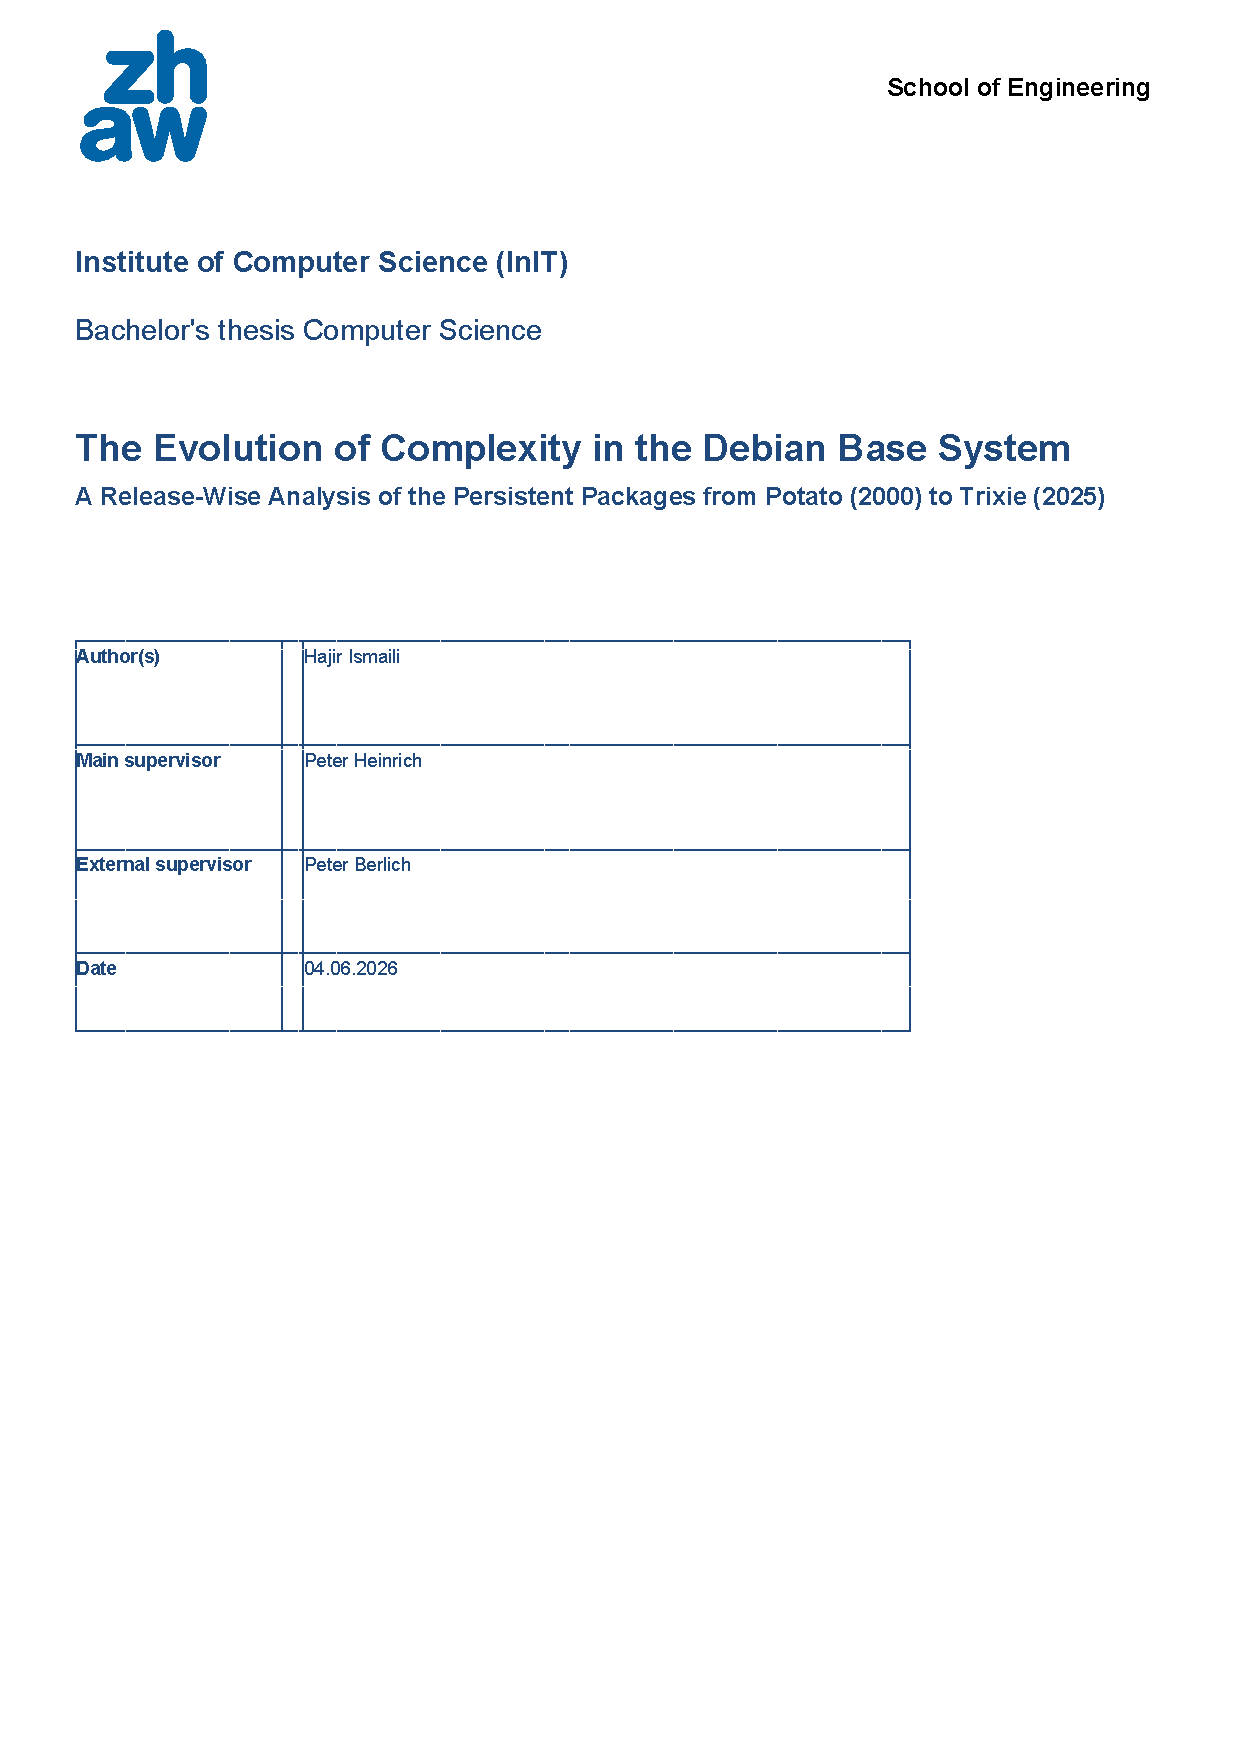
\includepdf[pages=-]{parts/01_front_matter/Title_page.pdf}
\clearpage

% English Abstract
\begin{abstract}
Software systems tend to grow as they evolve, yet how this growth manifests in the base of a long-lived Linux distribution has not been characterised systematically. This thesis provides a reproducible, release-wise characterisation of the persistent core of Debian's minbase installation, the minimal package set that \texttt{debootstrap} resolves for each release: the 25 source packages present in this set in at least 11 of the 13 stable releases from Potato (2000) to Trixie (2025). A containerised pipeline downloads each release's package indices and source archives and computes five metrics per release: installed size, dependency structure, lines of code, per-function cyclomatic complexity, and distribution-specific patch volume. The results describe growth by accretion. The persistent core grows roughly 5.3-fold in lines of code and roughly fourfold in installed size, while the median per-function cyclomatic complexity remains at 3 in every release and the median per-package dependency count at 1 in every release after Potato; the composition of the minbase changes chiefly through packaging structure rather than capability. The patch-volume metric is comparable only from the 3.0 (quilt) source format onward and declines within that window. The study is exploratory-descriptive and asserts no causal or correlational relationship between the dimensions. The pipeline and an interactive companion application are made publicly available to enable reproduction and extension of the analysis.

\vspace{6em} 

\noindent\textbf{Keywords:} Debian, software evolution, software bloat, software metrics, cyclomatic complexity, mining software repositories

\end{abstract}
\clearpage

% German Abstract (Zusammenfassung)
\selectlanguage{german}
\begin{abstract}
Softwaresysteme neigen dazu, im Laufe ihrer Entwicklung zu wachsen; wie sich dieses Wachstum in der Basis einer langlebigen Linux-Distribution äussert, ist jedoch wenig untersucht. Diese Arbeit liefert eine reproduzierbare, releaseweise Charakterisierung des persistenten Kerns der minbase-Installation von Debian, der minimalen Paketmenge, die \texttt{debootstrap} für jedes Release auflöst: der 25 Quellpakete, die in mindestens 11 der 13 stabilen Releases von Potato (2000) bis Trixie (2025) in dieser Menge enthalten sind. Eine containerisierte Pipeline lädt die Paketindizes und Quellarchive jedes Releases herunter und berechnet fünf Metriken pro Release: Installationsgrösse, Abhängigkeitsstruktur, Quelltextzeilen, zyklomatische Komplexität pro Funktion und das Volumen distributionsspezifischer Patches. Die Ergebnisse beschreiben ein Wachstum durch Anlagerung. Der persistente Kern wächst etwa um das 5,3-Fache in Quelltextzeilen und etwa um das Vierfache in der Installationsgrösse, während der Median der zyklomatischen Komplexität pro Funktion in allen Releases bei 3 verbleibt und der Median der Abhängigkeiten pro Paket in jedem Release nach Potato bei 1 liegt; die Zusammensetzung der minbase-Installation ändert sich vor allem durch die Paketierungsstruktur und nicht durch den Funktionsumfang. Die Patch-Metrik erweist sich erst ab dem Quellformat 3.0 (quilt) als vergleichbar und nimmt innerhalb dieses Fensters ab. Die Studie ist explorativ-deskriptiv angelegt und behauptet keine kausalen oder korrelativen Zusammenhänge zwischen den Dimensionen. Die Pipeline und eine interaktive Begleitanwendung werden zusammen mit den Ergebnissen veröffentlicht, um Reproduktion und Erweiterung zu ermöglichen.

\vspace{6em} 

\noindent\textbf{Schlüsselwörter:} Debian, Softwareevolution, Software-Bloat, Softwaremetriken, zyklomatische Komplexität, Mining Software Repositories

\end{abstract}
\clearpage
\selectlanguage{english}

% Table of Contents
\pagenumbering{roman}
\renewcommand{\contentsname}{Table of Contents}
\tableofcontents
\clearpage

% List of Figures and List of Tables (shared page)
\markboth{List of Figures and List of Tables}{}
\listoffigures
\bigskip
\listoftables
\clearpage

\pagenumbering{arabic}
% ========================== MAIN MATTER ===========================

\chapter{Introduction}\label{ch:introduction}
Software systems tend to grow in complexity and size as they evolve, a phenomenon that Lehman formalized in his Laws of Software Evolution~\cite{Lehman1980Laws}: actively used software must continually adapt to its environment, and that adaptation inevitably increased complexity unless deliberate effort was made to reduce it. Niklaus Wirth revisited this concern in 1995, arguing that the trend had persisted and that software's resource demands continued to outpace its functional improvements~\cite{Wirth1995Plea}. This long-term growth poses challenges to the core principles of the GNU Project philosophy, which emphasises the ability of users to read, understand, and extend the software they run~\cite{Sherlock2018OpenSS}. Empirical studies of software maintenance have further reported that increased complexity was associated with measurable increases in maintenance cost and defect density~\cite{nguyen2017impact}. Debian, one of the oldest and most widely used Linux distributions, is the basis for numerous derivative distributions, including Ubuntu; according to W3Techs, Debian and its derivatives collectively accounted for over 40\% of all Linux-powered websites~\cite{W3Techs2024Linux}. Changes in Debian's core packages therefore propagate into a significant share of contemporary computing infrastructure, which motivates a systematic, descriptive account of how those packages have developed since the distribution's earliest stable release.

\section*{Research Gap}
While the general phenomenon of increasing software size has been widely discussed, and longitudinal studies exist for individual software packages~\cite{molnar2020longitudinal}, no systematic descriptive account exists of how Debian's persistent core packages have developed across the distribution's full release history. In particular, no publicly available pipeline characterises installed size, inter-package dependency structure, lines of code, per-function cyclomatic complexity, and distribution-specific patch volume jointly across every stable Debian release. This thesis addresses that gap by building such a pipeline and applying it to every persistent package in the minbase installation across the 13 stable Debian releases from Potato (2000) to Trixie (2025). The work is framed as exploratory research: it describes what can be observed using the chosen set of tools and metrics, without claiming a causal or correlational relationship between the observed dimensions.

\section*{Research Questions}
Following the exploratory-descriptive framing above, this thesis addresses the following primary research question:

\begin{itemize}
    \item What does a reproducible release-wise analysis of the persistent packages in Debian's minbase installation, using an open-source tool pipeline, reveal about their development across all stable releases from Potato (2000) to Trixie (2025), characterised along the dimensions of installed size, dependency structure, lines of code, per-function cyclomatic complexity, and distribution-specific patch volume?
\end{itemize}

Two secondary questions sharpen the primary one:
\begin{itemize}
    \item How has the composition of Debian's minbase installation changed across releases, specifically which packages entered, which were removed, and which form the persistent core?
    \item How has the volume and file-level structure of distribution-specific patches maintained by Debian on top of upstream source code evolved across releases?
\end{itemize}

The research questions are deliberately descriptive. The thesis does not ask whether observed changes in one dimension are correlated with, caused by, or predictive of changes in another; such inferential claims would require larger samples, controlled comparisons, and tools beyond the scope of this work.

\section*{Method}
The methodological mode of this thesis is exploratory-descriptive: a phenomenon (the release-by-release development of Debian's persistent core packages) is characterised using a defined toolchain, and the characterisation itself is the contribution. The method of data collection is a release-wise analysis of every persistent package in the minbase installation, from which five metrics are extracted per release: installed size from the Debian \texttt{Packages} index, dependency edges from the \texttt{Depends} field of that same index, lines of code from the upstream source tarballs using \texttt{tokei}, distribution-specific patch volume from the Debian patch archive, and per-function cyclomatic complexity~\cite{CyclomaticComplexity} from the C and C++ source files of those tarballs using \texttt{pmccabe}. Because cyclomatic complexity is defined at the level of a single function rather than at the level of a package, package- and release-level quantities are always reported as aggregates (mean, median, maximum, sum) over the per-function measurements. The full pipeline is containerised with Docker and orchestrated by a Makefile to make the analysis reproducible. A detailed description of the data collection and analysis methodology is provided in \autoref{ch:method}.

\section*{Expected Output}
The deliverables of this thesis are a reproducible analysis pipeline together with the descriptive artefacts it produces when applied to the 13 stable Debian releases between 2000 and 2025. Concretely, these comprise:

\begin{itemize}
    \item A release-wise timeline of the minbase installation's package composition, reporting the package count of every release, resolving its largest movements package by package, and identifying the 25 source packages that form the persistent core.
    \item Per-release summary statistics and visualisations for installed size (minbase total and persistent subset), dependency structure (per-package dependency counts), lines of code (total and decomposed by programming language), per-function cyclomatic complexity (mean, median, maximum, and per-release distribution), and distribution-specific patch volume.
    \item A containerised pipeline of established open-source tools (\texttt{debootstrap}, \texttt{tokei}, \texttt{pmccabe}, \texttt{gnuplot}) and supporting shell and AWK scripts, released alongside the thesis and intended to be reproducible and extensible by other researchers.
    \item An interactive companion application, the Debian Bloat Explorer, built with the Streamlit framework, that reads the same per-release CSV files as the plotting scripts and supports drill-down into individual packages and releases for verifying and diagnosing the aggregate figures.\footnote{A hosted instance is publicly available at \url{https://debian-bloat-explorer.streamlit.app} (accessed 4 June 2026); source code and data availability are documented in \autoref{app:availability}.}
    \item A catalogue of figures (line charts, boxplots, stacked histograms, bar charts) that make the development of each metric visually accessible without themselves constituting substantive claims about the direction or magnitude of that development. The discussion chapter synthesises these descriptive findings and situates them against prior work; interpretation that goes beyond such synthesis, in particular any causal or correlational claim relating one dimension to another, is deferred to future work.
\end{itemize}

Additional per-package metrics such as the Maintainability Index~\cite{Coleman1994Using} were considered during scoping; they are not part of the current pipeline but represent a natural extension.

\section*{Relevance}
The relevance of this thesis lies in producing, and making reproducible, a descriptive baseline of how Debian's persistent core packages have developed since the distribution's earliest stable release. The pipeline and the resulting per-release artefacts are intended as a foundation: future work that wishes to investigate causal mechanisms behind complexity growth, to evaluate automated software de-bloating techniques~\cite{quach2018debloating}, or to compare Debian with other long-lived distributions can take the metrics and visualisations produced here as its starting point, rather than having to rebuild the data-collection pipeline from scratch.

\section*{Project Structure}
The thesis is structured as follows: the introduction establishes the context, research gap, and the exploratory-descriptive framing that guides the remainder of the work. The related work section reviews existing literature on software complexity metrics, studies of open-source software evolution, and prior analyses of Debian's package management system. The method section describes the data-collection and analysis pipeline in detail, including the tools used, the definition of the minbase installation, the identification of persistent packages, and the exact procedure for computing each metric. The results section presents the per-release artefacts produced by the pipeline: summary statistics, figures, and composition timelines. The discussion section reviews what can and cannot legitimately be said from those artefacts, names the limitations of the approach, and identifies directions for future work. The conclusion summarises the artefacts produced and the scope of the claims they support.
\clearpage

\chapter{Related Work}\label{ch:relatedwork}
Research into software growth, complexity, and distribution-level maintenance spans several distinct communities. This chapter situates the present study within four adjacent strands of literature: the empirical validation of software evolution laws, longitudinal case studies of the Linux kernel and other open source systems, structural studies of Debian and other Linux distributions, and quantitative complexity metrics for software quality. The review intentionally focuses on prior art and methodological precedents, independent of the findings presented in later chapters.

\section{Laws of Software Evolution}
\label{sec:rw_evolution}

The theoretical foundation for studying long-term software change originates in the work of Lehman, whose Laws of Software Evolution postulate that actively used software systems continually change, grow in size, and increase in complexity unless explicit effort is invested in reducing it~\cite{Lehman1980Laws}. Wirth subsequently argued that this tendency had become a structural problem in the software industry, driven by the ease with which hardware advances absorbed inefficient designs, and called for a return to lean software engineering~\cite{Wirth1995Plea}.

Subsequent empirical research has sought to test Lehman's laws against real-world software. Neamtiu et al. analyzed 653 official releases of seven open source projects across a combined 69 years of evolution and reported partial support for the laws, with growth and continuing change emerging as the most robustly confirmed propositions~\cite{neamtiu2009towards}. Vasa examined distributions of software metrics across successive releases and likewise found consistent evidence for continuing change, self-regulation, conservation of familiarity, and continuing growth, while remaining unable to substantiate several other laws~\cite{vasa2010growth}. More recently, Smajić et al. revisited the laws through a comparative lens, contrasting open and closed source projects and suggesting that licensing models shape the observed evolution dynamics~\cite{smajic2025evolution}. Taken together, these studies establish empirical validation of Lehman's laws as an active and methodologically varied line of inquiry, but they largely focus on individual projects rather than on the aggregate evolution of a complete software distribution.

\section{Longitudinal Studies of the Linux Kernel}
\label{sec:rw_kernel}

The Linux kernel has served as the canonical subject for empirical studies of open source evolution. Godfrey and Tu examined roughly a decade of kernel releases and reported a super-linear growth rate in lines of code, contradicting the expectation that large systems slow as they mature~\cite{godfrey2000linux}. Koren extended this analysis to 534 kernel versions and contrasted growth in stable and development branches, observing that development versions accumulated code more aggressively than their stable counterparts~\cite{koren2006linux}.

Israeli and Feitelson conducted the most extensive kernel study to date, analyzing 810 kernel versions across 14 years using several of the metrics also relevant to the present thesis, including lines of code, function counts, and McCabe's cyclomatic complexity~\cite{israeli2010linux}. Their results support several of Lehman's laws and yield a particularly relevant observation: although total kernel complexity increases over time, the average cyclomatic complexity of individual functions decreases, primarily because new code is introduced in the form of many small, low-complexity functions. This result is the closest methodological precedent for the present thesis: it demonstrates that function-level complexity metrics can be aggregated across long release histories, and that a complexity trend can only be read from total and average measures side by side.

\section{The Debian and Linux Distribution Ecosystem}
\label{sec:rw_distribution}

A separate strand of research treats Linux distributions as ecosystems rather than as individual programs. LaBelle and Wallingford modelled inter-package dependency networks in Debian and demonstrated that these networks exhibit scale-free structural properties characteristic of complex networks~\cite{interPackageDependency}. De Sousa et al. analyzed the dependency graph of over 18{,}000 Debian packages and confirmed its scale-free nature, further identifying community structure that aligned with the organizational boundaries of maintenance teams~\cite{sousa2009debian}. Horváth extended the comparison to Ubuntu, Debian, and Arch Linux, studying how edges accumulate between successive distribution versions and providing evidence for preferential attachment at the ecosystem level~\cite{horvath2012linuxdeps}.

More recent work has reconstructed the historical evolution of Debian directly from archived mirrors. Tang et al. collected snapshots of every Debian release and built dependency graphs for each, enabling an analysis of compatibility and security issues that arise when the ecosystem moves between releases~\cite{tang2024frozen}. Their study is methodologically adjacent to the present thesis in its use of archived Debian metadata for longitudinal analysis, although its focus is on the consequences of frozen package versions rather than on the internal complexity of the packages themselves.

Distribution-specific maintenance work has also attracted empirical attention. Becker et al. introduced the CoLiS platform to systematically analyze over twenty-seven thousand Debian maintainer scripts and uncovered more than 150 policy violations; the size of this script corpus alone indicates how much distribution-level maintenance lies beyond the upstream code itself~\cite{becker2022colis}. Lin et al. studied upstream bug management and vulnerability handling across Debian and Fedora, quantifying the fraction of fixes contributed locally by distribution maintainers rather than propagated from upstream projects~\cite{lin2022upstream,lin2023vulnerability}. These studies motivate the measurement of distribution-specific patch volume as an indicator of the effort that a distribution invests in adapting upstream software, a theme this thesis takes up for persistent Debian packages.

\section{Complexity Metrics for Software Quality}
\label{sec:rw_metrics}

The quantitative metrics used to characterize software complexity have been studied extensively. McCabe's cyclomatic complexity, which counts the number of linearly independent paths through a function's control flow graph, remains among the most widely applied measures of structural complexity and is routinely used as a proxy for testability and maintainability~\cite{CyclomaticComplexity}. Empirical research has associated rising complexity with increased maintenance cost and higher defect density in both open source and proprietary codebases~\cite{nguyen2017impact}.

Several studies have applied complexity metrics to concrete long-lived software systems. Ronchieri et al. assessed the cyclomatic complexity and related measures of Geant4, a large scientific simulation toolkit, to establish a quality baseline and identify modules at risk of future maintenance problems~\cite{ronchieri2016software}. Molnar and Motogna conducted a longitudinal evaluation of maintainability across multiple open source systems, tracking aggregate indices across many releases and demonstrating that distribution-level metric trends can diverge from individual project trends~\cite{molnar2020longitudinal}. Sherlock et al. surveyed the broader risks of open source adoption, framing metric-based monitoring as one component of risk management in software supply chains~\cite{Sherlock2018OpenSS}. These works collectively establish the precedent for using function-level complexity metrics at scale, while leaving largely unaddressed the question of how such metrics evolve across a complete Linux distribution over decades.

\section{Synthesis}
\label{sec:rw_synthesis}

The four strands leave a specific gap. The empirical validations of Lehman's laws and the longitudinal kernel studies measure individual software projects, whereas the distribution-level studies model dependency networks or cross-release compatibility without measuring the internal size and complexity of the packages themselves; the metric studies, in turn, apply complexity measurement to single systems rather than across a distribution's release history. None of the strands therefore produces a longitudinal, multi-metric account of the packages that constitute a distribution's base system. Research on automated software de-bloating approaches the same concern from the opposite direction, removing unneeded code from deployed software~\cite{quach2018debloating,brown2023sokdebloating}, and presupposes measurement baselines that identify where and how bloat accumulates. The present thesis supplies such a baseline for the persistent core of Debian's minbase installation, combining the function-level complexity measurement established by the kernel studies with the release-wise, archive-based reconstruction used by the distribution studies.

\clearpage

\chapter{Method}\label{ch:method}
This chapter describes the methodology used to characterise the persistent packages in Debian's minbase installation across releases. The analysis spans the 13 stable Debian releases from Potato (2000) to Trixie (2025), covering over 25 years of distribution development. The approach is exploratory-descriptive: the aim is to produce, for every release, a comparable set of measurements and visualisations that describe the state of the persistent core, rather than to test a specific hypothesis about how or why it has changed. The entire pipeline is automated through shell scripts orchestrated by a Makefile and executed inside a Docker container to ensure reproducibility.

\section{Overview}
\label{sec:method-overview}

The methodology follows a four-stage pipeline: data acquisition, parsing and package identification, metric computation, and visualization (\autoref{fig:pipeline-overview}). First, package metadata and source archives are downloaded from official Debian mirrors. Second, the metadata is parsed into structured formats, the minbase installation is defined for each release, and packages that persist across releases are identified. Third, five quantitative metrics are computed for these persistent packages: installed size, dependency count, lines of code, distribution-specific patch volume, and cyclomatic complexity. Finally, the results are visualized as trend plots across all releases.

\begin{figure}[ht]
  \centering
  \begin{tikzpicture}[
      stage/.style={draw, rounded corners, align=center, minimum height=1.1cm, text width=2.7cm, font=\small\bfseries},
      artefacts/.style={align=center, font=\scriptsize, text width=2.9cm},
      flow/.style={-{Stealth[length=2.5mm]}, semithick}
    ]
    \node[stage]                       (acq)   {Data\\acquisition};
    \node[stage, right=0.7cm of acq]   (parse) {Parsing and\\identification};
    \node[stage, right=0.7cm of parse] (metr)  {Metric\\computation};
    \node[stage, right=0.7cm of metr]  (vis)   {Visualization};

    \draw[flow] (acq)   -- (parse);
    \draw[flow] (parse) -- (metr);
    \draw[flow] (metr)  -- (vis);

    \node[artefacts, below=0.3cm of acq]   {\texttt{Packages.gz},\\ \texttt{Sources.gz},\\ source archives};
    \node[artefacts, below=0.3cm of parse] {normalised CSVs,\\ minbase lists,\\ persistent set};
    \node[artefacts, below=0.3cm of metr]  {size, dependencies,\\ lines of code, patches,\\ complexity};
    \node[artefacts, below=0.3cm of vis]   {per-release\\ figures};
  \end{tikzpicture}
  \caption[Overview of the analysis pipeline.]{Overview of the four-stage analysis pipeline. Each box is one stage and each arrow the flow of artefacts between consecutive stages; the label beneath a box names the principal artefacts that the stage downloads or produces. The pipeline runs inside a Docker container and is orchestrated by a Makefile.}
  \label{fig:pipeline-overview}
\end{figure}

\section{Dataset and Scope}
\label{sec:dataset}

The dataset comprises 13 stable Debian releases, listed in Table~\ref{tab:releases}. These releases span from version 2.2 (Potato, released 2000) to version 13 (Trixie, released 2025), covering over 25 years of distribution development. Releases prior to Potato are excluded because \texttt{debootstrap}~\cite{debootstrap} does not provide bootstrap scripts for those releases, and their source archives lack consolidated machine-readable indices (\texttt{Sources.gz}), which the pipeline requires for automated analysis. Both binary and source package indices are available for all 13 releases.

\begin{table}[ht]
  \centering
  \caption{Debian releases included in the analysis.}
  \label{tab:releases}
  \begin{tabular}{llcl}
    \hline
    Codename & Version & Year & Architecture \\
    \hline
    Potato   & 2.2  & 2000 & i386  \\
    Woody    & 3.0  & 2002 & i386  \\
    Sarge    & 3.1  & 2005 & i386  \\
    Etch     & 4.0  & 2007 & i386  \\
    Lenny    & 5.0  & 2009 & i386  \\
    Squeeze  & 6.0  & 2011 & amd64 \\
    Wheezy   & 7.0  & 2013 & amd64 \\
    Jessie   & 8.0  & 2015 & amd64 \\
    Stretch  & 9    & 2017 & amd64 \\
    Buster   & 10   & 2019 & amd64 \\
    Bullseye & 11   & 2021 & amd64 \\
    Bookworm & 12   & 2023 & amd64 \\
    Trixie   & 13   & 2025 & amd64 \\
    \hline
  \end{tabular}
\end{table}

The analysis targets the \texttt{main} component of each release, which contains only free software as defined by the Debian Free Software Guidelines. Releases from Potato through Lenny are analyzed on the i386 architecture, while Squeeze onward are analyzed on amd64, reflecting the architecture transition that occurred in the Debian project around 2011. Package metadata is retrieved from \texttt{archive.debian.org} for historical releases and from \texttt{deb.debian.org} for the most recent releases still hosted on the primary mirror.

\section{Defining the Minbase Installation}
\label{sec:minbase}

A central concept in this analysis is the \emph{minbase installation}, the package set produced by \texttt{debootstrap}~\cite{debootstrap} when invoked with the \texttt{-{}-variant=minbase} option. It contains every binary package marked as \texttt{Essential: yes} or \texttt{Priority: required} in the release's package index, together with the transitive closure of their declared dependencies~\cite{debianPolicy}. With the \texttt{-{}-print-debs} flag, \texttt{debootstrap} reports this list without performing an actual installation, which allows the pipeline to reproduce the exact minbase set for every release from Potato (2000) to Trixie (2025). Because all 13 releases in the dataset are supported by \texttt{debootstrap}, the definition is applied consistently across the entire scope of the analysis.

The term \emph{minbase installation} is chosen deliberately, rather than the looser phrase ``minimal installation'', because Debian distinguishes several distinct base tiers of differing size. Table~\ref{tab:install-tiers} summarizes them, ordered from smallest to largest. Each tier adds packages on top of the previous one; only the tiers that include a kernel image and a bootloader can boot on bare hardware.

\begin{table}[ht]
  \centering
  \caption{Debian installation tiers, ordered by increasing size.} 
  \label{tab:install-tiers}
  \footnotesize
  \begin{tabular}{p{0.35\textwidth}p{0.48\textwidth}c}
    \hline
    Tier & Contents & Bootable  \\
    \hline
    \texttt{debootstrap -{}-variant=buildd}    & Subset of minbase tailored for package-build chroots & no \\
    \hline
    \texttt{debootstrap -{}-variant=minbase}   & \texttt{Essential: yes} plus \texttt{Priority: required} and transitive dependencies & no \\
    \hline
    \texttt{debootstrap} (default variant)     & Minbase plus all \texttt{Priority: important} packages (e.g., \texttt{apt}, basic network tools, \texttt{less}) & no \\
    \hline
    Installer ``base system''                  & Default debootstrap plus kernel, bootloader, and firmware & yes \\
    \hline
    Installer plus ``standard'' task           & Base system plus the standard system utilities task & yes \\
    \hline
  \end{tabular}
\end{table}

The minbase tier is not bootable on bare hardware because it contains no kernel image, no bootloader, and no hardware-specific firmware. It is designed instead to populate chroot environments and container base images; the official \texttt{debian:*-slim} Docker images are built from a package set close to this tier. Measuring the minbase tier, rather than a full installer image, removes two major confounders from the longitudinal comparison: the size of the Linux kernel (an upstream concern, not a Debian packaging decision) and the choice of bootloader (which varies across hardware eras). All subsequent metrics in this thesis are computed with respect to the minbase set and its persistent subset (\autoref{sec:persistent}).

\section{Identifying Persistent Packages}
\label{sec:persistent}

Not all packages in the minbase installation are suitable for longitudinal complexity analysis. Packages that appear only in a few releases provide insufficient data for trend observation. Therefore, the analysis focuses on \emph{persistent packages}: source packages that are present in the minbase installation across a large majority of releases.

The identification proceeds in three steps. First, for each release, the binary packages in the minbase installation are mapped to their corresponding source packages using the \texttt{Source} field from the parsed package metadata. Second, package aliases are resolved to account for historical renames; for example, the source package \texttt{shellutils} was merged into \texttt{coreutils} in later releases. An alias configuration file maps these historical names to their current equivalents. Third, the number of releases in which each source package appears is counted. Packages present in at least 80\% of all releases (at least 11 out of 13) are classified as persistent. This threshold ensures that only packages with a substantial longitudinal presence are included, while allowing for the fact that some packages did not exist in the earliest releases.

Applying the procedure to the 13 releases yields the 25 source packages listed in Table~\ref{tab:persistent-packages}. Twenty of them appear in every release (13/13); the remaining five clear the threshold with 11 or 12 appearances. This set constitutes the study population for all subsequent metrics (installed size of the persistent subset, lines of code, cyclomatic complexity, and patch volume).

\begin{table}[ht]
  \centering
  \caption[Persistent source packages analyzed in this thesis.]{Persistent source packages analyzed in this thesis. A package qualifies if its source name appears in the minbase set of at least 11 of 13 releases ($\geq 80\%$).}
  \label{tab:persistent-packages}
  \begin{tabular}{lc@{\qquad}lc@{\qquad}lc}
    \hline
    Package & $n$/13 & Package & $n$/13 & Package & $n$/13 \\
    \hline
    \texttt{acl}          & 11 & \texttt{dpkg}       & 13 & \texttt{pam}        & 13 \\
    \texttt{attr}         & 11 & \texttt{e2fsprogs}  & 12 & \texttt{perl}       & 12 \\
    \texttt{base-files}   & 13 & \texttt{findutils}  & 13 & \texttt{sed}        & 13 \\
    \texttt{base-passwd}  & 13 & \texttt{glibc}      & 13 & \texttt{shadow}     & 13 \\
    \texttt{bash}         & 13 & \texttt{grep}       & 13 & \texttt{sysvinit}   & 13 \\
    \texttt{coreutils}    & 13 & \texttt{gzip}       & 13 & \texttt{tar}        & 13 \\
    \texttt{debconf}      & 13 & \texttt{hostname}   & 13 & \texttt{util-linux} & 13 \\
    \texttt{debianutils}  & 13 & \texttt{mawk}       & 13 &                     &    \\
    \texttt{diffutils}    & 11 & \texttt{ncurses}    & 13 &                     &    \\
    \hline
  \end{tabular}
\end{table}

\section{Data Acquisition}
\label{sec:acquisition}

Data acquisition proceeds in three stages, corresponding to the three types of artifacts required for the analysis.

\subsection*{Package Metadata}
For each release, the compressed binary package index (\texttt{Packages.gz}) is downloaded from the appropriate Debian mirror. This file contains one stanza per binary package, with fields including the package name, version, priority, section, installed size, download size, and dependency list. The file is decompressed and stored locally for parsing.

\subsection*{Source Package Indices}
For each release, the \texttt{Sources.gz} file is downloaded. Each stanza in this file describes a source package and lists the associated upstream tarball (\texttt{.orig.tar.*}) and Debian-specific archive (\texttt{.debian.tar.*} or \texttt{.diff.gz}), along with their file paths relative to the mirror root.

\subsection*{Source Archives}
For each persistent package in each release, the upstream source tarball and the Debian-specific patch archive are downloaded. The upstream tarball contains the original source code as released by the upstream maintainer. The Debian-specific archive contains the packaging metadata and any patches applied by Debian maintainers to adapt the software for the distribution. These archives are required for lines-of-code counting, complexity analysis, and patch volume measurement.

All downloads use retry logic with retry delays (up to three attempts) and a 120-second timeout per request. Downloads are idempotent: files already present on disk are not re-downloaded.

\section{Data Parsing}
\label{sec:parsing}

The raw Debian metadata files use a stanza-based format that is not directly suitable for quantitative analysis. Each \texttt{Packages} file is parsed into a comma-separated values (CSV) file using AWK, extracting the fields: package name, source package, version, priority, section, installed size, download size, and dependencies. Dependency lists, which use commas as separators in the original format, are converted to semicolons to preserve CSV integrity. Field matching is performed case-insensitively to accommodate formatting variations in the earliest releases.

Similarly, each \texttt{Sources} file is parsed into a CSV containing the source package name, version, directory path, and the filenames and sizes of the upstream and Debian-specific archives. These parsed CSVs serve as the structured input for all subsequent analysis steps.

\section{Metrics}
\label{sec:metrics}

Five quantitative metrics are computed for the persistent packages across all releases. Each metric captures a different dimension of software complexity or distribution maintenance effort.

\subsection{Installed Size}
\label{sec:metric-size}

The installed size of a package, as reported in the \texttt{Installed-Size} field of the package metadata, represents the disk space (in kilobytes) consumed by the package after installation. For each release, two aggregate values are computed: the total installed size of the minbase installation, and the total installed size of only the persistent packages within the minbase installation. This metric provides a measure of the overall footprint growth of the base system.

\subsection{Dependency Count}
\label{sec:metric-deps}

The dependency count for each package is derived from its \texttt{Depends} field, which lists the other packages required for the package to function. Each entry in the dependency list is counted as one dependency edge, where alternative dependencies (expressions of the form \texttt{a | b}) are treated as a single dependency edge. For each release, the per-package dependency counts are recorded over all packages in the minbase installation (rather than over the persistent subset only), because dependency structure is a graph-level property of the minbase as a whole: restricting the computation to the fixed persistent population would obscure the arrival of new hub packages such as \texttt{systemd} that enter the required set mid-timeline. The resulting per-release distributions are visualised as boxplots so that the central tendency (median), the spread (interquartile range), and the extreme hub packages (outliers above the whiskers) are readable simultaneously. This metric quantifies the interconnectedness of the minbase installation and is an indicator of system-level coupling~\cite{interPackageDependency}.

\subsection{Lines of Code}
\label{sec:metric-nloc}

The number of lines of code (NLOC) is measured using \texttt{tokei}~\cite{tokei}, a source code statistics tool that distinguishes between code lines, comment lines, and blank lines. For each persistent package in each release, the upstream source tarball is extracted and analyzed with \texttt{tokei}. The tool automatically detects programming languages and reports per-language statistics, so every language present in a tarball, whether compiled or interpreted, contributes to the count. Results are aggregated at two levels: per package (total code, comments, and blanks across all languages) and per release (total code volume and language composition). To produce a consistent language breakdown, related language variants are first normalized: C header files are merged with C, Bash and Zsh are merged into a single Shell category, and GNU-style assembly is merged with Assembly. The breakdown then records C, Shell, Assembly, Python, and Perl as individual categories and groups all remaining languages under an ``Other'' category.

\subsection{Patch Volume}
\label{sec:metric-patches}

Debian maintainers apply patches to upstream source code to fix bugs, adapt software to Debian policies, or backport security fixes. The volume of these distribution-specific patches is measured for each persistent package by examining the Debian-specific archive. The form of this archive is determined by the source-package format that the package declares~\cite{debsrc3quilt}. Under the older \texttt{1.0} format, all distribution-specific material, that is, the packaging files under \texttt{debian/} together with any modifications to upstream files, is bundled into a single \texttt{.diff.gz} file. Under the \texttt{3.0 (quilt)} format, named after the \texttt{quilt} patch-management tool, the packaging metadata is carried in a \texttt{.debian.tar.*} archive and modifications to upstream source are kept as individual named patch files in unified diff format under \texttt{debian/patches/}. For each package, three values are recorded: the size of the Debian archive in bytes, the total number of patch lines across all patch files, and the number of individual patch files. Per-release aggregates include the total patch lines, the average patch lines per package, and the number of packages that carry at least one patch.

\subsection{Cyclomatic Complexity}
\label{sec:metric-cc}

Cyclomatic complexity (CC) measures the number of linearly independent paths through a function's control flow graph~\cite{CyclomaticComplexity}. A higher CC value indicates more complex branching logic and, by extension, greater difficulty in testing and maintaining the function. CC is computed using \texttt{pmccabe}~\cite{pmccabe}, a static analysis tool for C and C++ source code. For each persistent package, all C and C++ source files (\texttt{.c}, \texttt{.h}, \texttt{.cc}, \texttt{.cpp}, \texttt{.cxx}) are extracted from the upstream tarball and analyzed. The tool reports the modified cyclomatic complexity for each function, which differs from the classic McCabe count in treating a multi-way \texttt{switch} statement as a single decision point rather than counting each \texttt{case} label separately; this convention avoids inflating the complexity of the \texttt{switch}-heavy C code that comprises much of the Debian base system.

Per-package aggregates include the number of functions analyzed, the average CC, the maximum CC, and the sum of all CC values. Per-release aggregates include the total number of functions, the average CC, the maximum CC, and the median CC. The median is computed from the sorted list of all function-level CC values in the release and is reported alongside the mean to reduce the influence of outlier functions with exceptionally high complexity.

Because \texttt{pmccabe} parses only C and C++ source, the complexity metric covers the subset of persistent packages that ship such source. Packages implemented entirely in other languages yield no complexity measurement. Two persistent packages are affected: \texttt{debconf}, which is written in Perl, and \texttt{base-files}, which consists of shell fragments and static configuration data. Neither contains C or C++ source, so neither contributes to the complexity results, although both are still measured for the remaining metrics, including lines of code. The consequences of this language restriction for the interpretation of the complexity trends are addressed in Section~\ref{sec:limitations}.

\section{Reproducibility}
\label{sec:reproducibility}

The entire pipeline is containerized using Docker. The Docker image is based on Debian Bookworm and includes all required tools: \texttt{curl} and \texttt{gzip} for downloads, \texttt{gawk} for parsing, \texttt{debootstrap} for minbase installation resolution, \texttt{tokei} for code counting, \texttt{pmccabe} for complexity analysis, and \texttt{gnuplot} for visualization. The pipeline is orchestrated by a Makefile that enforces the correct execution order through dependency declarations. A single command (\texttt{make all}) builds the Docker image, executes the full pipeline, and produces all output files.

All intermediate results are cached: parsed CSVs, minbase lists, and analysis outputs are preserved between runs, and downloads skip files that already exist on disk. Output figures are placed in a versioned directory named after the current Git commit hash, enabling traceability between specific pipeline outputs and the code that produced them.

\section{Interactive Companion Application}
\label{sec:companion-app}

Alongside the batch pipeline, an interactive companion application was developed to support verification and diagnosis of the aggregate figures. The application, the Debian Bloat Explorer, is implemented with the Streamlit framework~\cite{streamlit} and reads the same per-release CSV files that the \texttt{gnuplot} scripts consume, so that the static figures and the interactive views are guaranteed to draw on identical data. It provides four views: a release timeline of the aggregate metrics, a per-package explorer that traces every metric for a single source package across all releases, a snapshot of a single release's minbase installation, and a comparison of two releases. The per-package and per-release granularity that the application exposes is used in \autoref{sec:webapp} to distinguish genuine changes in Debian from artefacts of the measurement, which the release-level aggregates alone cannot resolve.

\clearpage

\chapter{Results}\label{ch:results}
This chapter presents the descriptive artefacts produced by applying the pipeline of \autoref{ch:method} to the 13 stable Debian releases from Potato (2000) to Trixie (2025). Consistent with the exploratory-descriptive framing of the research question, each metric is reported as a release-wise series, and the figures describe what is observed rather than asserting a causal or correlational relationship between dimensions. \autoref{sec:webapp} first establishes the provenance and reliability of the measurements and isolates the one metric whose comparability is restricted. The subsequent sections then characterise the base system along the axes of the research question in turn: the composition of the minbase installation, which addresses the secondary research question (\autoref{sec:composition}); installed size (\autoref{sec:results-size}); dependency structure (\autoref{sec:results-deps}); lines of code (\autoref{sec:results-loc}); per-function cyclomatic complexity (\autoref{sec:results-cc}); and distribution-specific patch volume (\autoref{sec:results-patch}).

\section{Interactive Data Exploration}
\label{sec:webapp}

The metrics defined in Chapter~\ref{ch:method} are rendered by the pipeline as a fixed set of per-release plots. These static figures summarise each metric at the granularity of a whole release, which is the appropriate level for the longitudinal trends that the research question targets. During review of the plots, however, several discontinuities appeared that could not be diagnosed from a release-level aggregate alone. The earliest pipeline runs, for example, showed an abrupt increase in lines of code between Wheezy and Jessie and isolated zero-valued segments in individual per-package trajectories (\autoref{fig:nloc-artefact}). Determining whether such a feature reflects a genuine change in Debian or an artefact of the measurement requires inspecting the contributing packages and releases individually, which a static aggregate plot does not support.

\begin{figure}[ht]
  \centering
  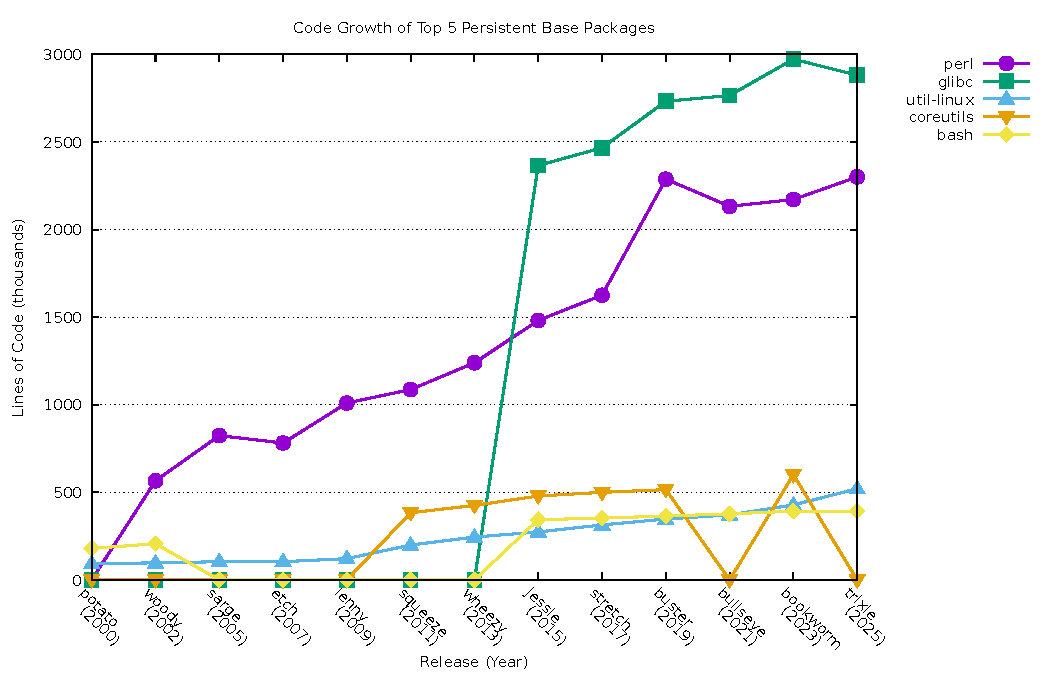
\includegraphics[width=\textwidth]{persistent_growth_artefact.pdf}
  \caption[Code growth of the five largest persistent base packages, from an early pipeline run.]{Lines of code for the five largest persistent base packages (\texttt{perl}, \texttt{glibc}, \texttt{util-linux}, \texttt{coreutils}, and \texttt{bash}), measured with \texttt{tokei} across the stable releases from Potato (2000) to Trixie (2025). Each curve traces one source package; the vertical axis gives total lines of code in thousands. The plot is taken from an early pipeline run and exhibits two measurement artefacts: a series that reads zero until it jumps abruptly at Jessie (\texttt{glibc}), and a series that falls to zero in individual releases (\texttt{coreutils}). These features are artefacts of the measurement rather than properties of the source code.}
  \label{fig:nloc-artefact}
\end{figure}

To enable this inspection, the interactive companion application described in \autoref{sec:companion-app}, the Debian Bloat Explorer, was used. Because it reads the same CSV files that the plotting scripts consume, its views and the static figures are guaranteed to draw on identical data. The per-package explorer isolates the contribution of one package at a time and was therefore used to diagnose the discontinuities.

Applying this tool resolved the first class of discontinuities and revealed a second. The lines-of-code discontinuity and the zero-valued segments were traced to three independent pipeline defects, namely the improper extraction of nested repacked tarballs, unresolved source-package aliases, and a detached signature file overwriting its tarball, and were corrected; after the fix the affected series grow smoothly and monotonically. The corrected aggregates therefore contain no remaining artefact of this kind. The interactive exploration of individual packages then exposed a second, qualitatively distinct inconsistency, one that the aggregate plots had concealed rather than introduced: the Debian patch-volume metric is not comparable across the release at which Debian changed its source-package format.

\FloatBarrier
\subsection{A Measurement Inconsistency in the Patch-Volume Metric}
\label{sec:patch-inconsistency}

The per-package explorer was used to examine \texttt{bash}, whose patch-volume series behaves anomalously. The number of Debian patch lines rises from roughly 9{,}000 in Potato to a peak of 63{,}000 in Sarge and then falls to 626 in Trixie (\autoref{fig:bash-patch-lines}), while the package's lines of code rise smoothly across the same period. Inspecting the historical source packages retrieved from the Debian snapshot archive, a timestamped store of every package version the project has distributed~\cite{debianSnapshot}, explains the discrepancy.

\begin{figure}[ht]
  \centering
  \setlength{\fboxsep}{0pt}%
  \setlength{\fboxrule}{0.4pt}%
  {\color{black!40}\fbox{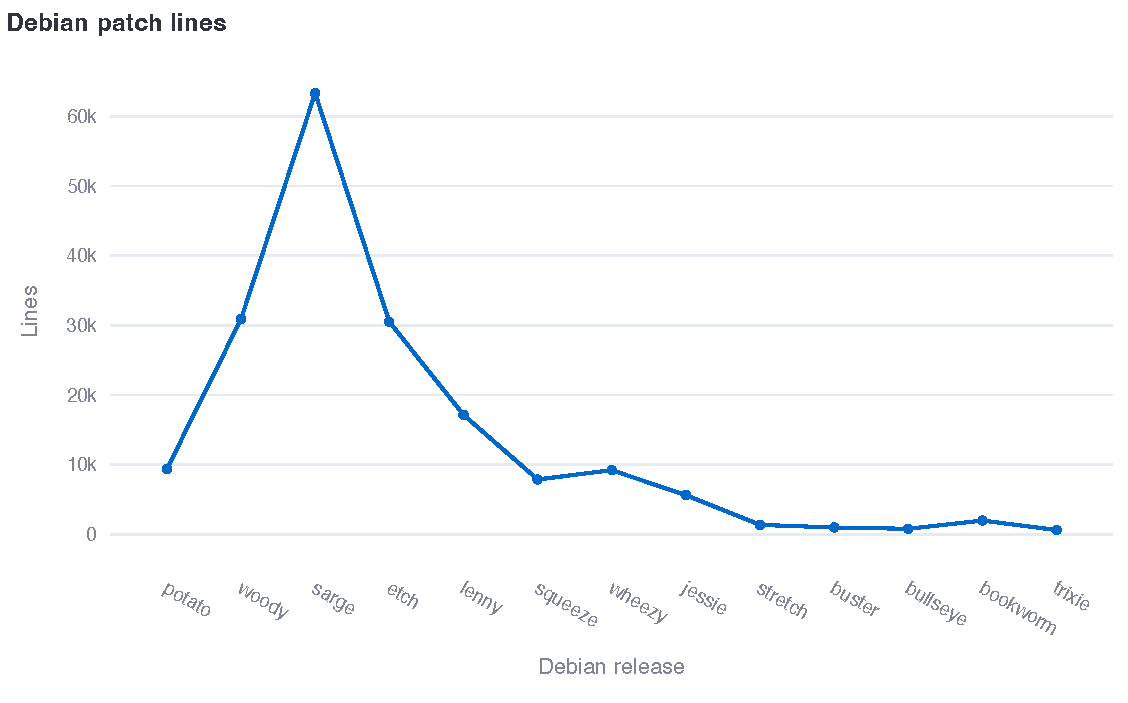
\includegraphics[width=\dimexpr\textwidth-2\fboxrule\relax]{bash-patch-lines.pdf}}}%
  \caption[Debian patch-line count for \texttt{bash} across releases.]{Debian patch-line count for \texttt{bash} across the stable releases from Potato to Trixie, shown in the per-package view of the Debian Bloat Explorer. The vertical axis counts the total number of lines in \texttt{bash}'s Debian-specific patch archive for each release: the single \texttt{.diff.gz} file under the \texttt{1.0} source format, and the files under \texttt{debian/patches/} under the \texttt{3.0 (quilt)} format.}
  \label{fig:bash-patch-lines}
\end{figure}

Until Jessie, Debian packaged \texttt{bash} in the \texttt{1.0} source format, in which all distribution-specific material is carried in a single \texttt{.diff.gz} file, and the patch-volume metric counts the lines of this file. Decomposing the file by content category (\autoref{tab:bash-patch-decomposition}) shows that the headline counts are dominated by material that does not modify the upstream source code. In Woody, 22{,}000 of the roughly 31{,}000 lines are an autotools build cache directory that the maintainer included in the diff. In Sarge, 45{,}000 lines are a single patch embedding the entire \texttt{bashdb} debugger project, a feature that was built only briefly and then disabled because breakpoints did not halt execution~\cite{bts224573}, and a further 13{,}000 lines are shell completion scripts. Across Potato to Lenny, the patches that genuinely modify upstream code never exceed roughly 11{,}000 lines in any release. The peak at Sarge arises because it is the only release in which the embedded debugger and a large completion-script collection are present at the same time.

\begin{table}[ht]
  \centering
  \caption[Principal components of the \texttt{bash} \texttt{.diff.gz}.]{Principal components of the \texttt{bash} \texttt{.diff.gz} under the \texttt{1.0} source format, in thousands of lines. The listed rows are the dominant contributors rather than an exhaustive partition; the remaining lines are \texttt{configure}-script regeneration, examples, and other files below \texttt{debian/}.}
  \label{tab:bash-patch-decomposition}
  \begin{tabular}{lrrrrr}
    \hline
    Component & Potato & Woody & Sarge & Etch & Lenny \\
    \hline
    autotools build cache        & ---  & 22.2 & ---  & ---  & ---  \\
    Embedded \texttt{bashdb}      & ---  & ---  & 44.7 & 0.6  & 0.6  \\
    Completion scripts            & ---  & 5.3  & 12.9 & 17.5 & 0.0  \\
    Upstream code-fix patches     & 4.4  & 1.1  & 2.5  & 7.9  & 10.6 \\
    Changelog and packaging       & 1.4  & 2.1  & 3.2  & 4.5  & 5.9  \\
    \hline
    Total \texttt{.diff.gz}       & 9.4  & 30.9 & 63.3 & 30.5 & 17.2 \\
    \hline
  \end{tabular}
\end{table}

The subsequent decline is likewise an artefact of packaging rather than of reduced modification. The completion scripts were moved into a separate source package in Lenny~\cite{bashChangelog}, and from Jessie onward \texttt{bash} was packaged in the \texttt{3.0 (quilt)} source format~\cite{debsrc3quilt}, which the Debian archive has accepted since 2009~\cite{ddaNewFormats2009} and which had become the most widely used format by 2011~\cite{hertzog2011quilt}. This format separates packaging metadata from the patch set and retains only named, purpose-specific patches under \texttt{debian/patches/} following the DEP-3 tagging convention, a Debian Enhancement Proposal that standardises a metadata header recording each patch's description, origin, and upstream-forwarding status~\cite{dep3}. The drop from 30{,}000 patch lines in Etch to 5{,}600 in Jessie therefore reflects a change in what the metric captures, not a reduction in Debian's modifications to \texttt{bash}.

The \texttt{bash} case indicates that the limitation extends to other packages. Because the \texttt{1.0} format bundles the entire \texttt{debian/} directory into a single diff~\cite{debsrc3quilt}, any package measured in that era is liable to carry patch-line counts inflated by changelogs, documentation, completion scripts, and other non-code material, so the metric is meaningfully comparable only within the \texttt{3.0 (quilt)} era from Jessie onward. The patch-volume series is consequently interpreted only within this later window. The case also illustrates why release-level aggregates are insufficient for diagnosing such inconsistencies: the artefact is invisible in the aggregate, which reports a single patch-line total per release, and became apparent only when the per-package composition could be inspected directly.

\section{Composition of the Minbase Installation}
\label{sec:composition}

The first dimension addresses the secondary research question of how the minbase installation has changed across releases. \autoref{fig:package-count} plots the number of binary packages that \texttt{debootstrap} resolves for the minbase variant of each release. The series is non-monotonic. It begins at 46 packages in Potato, dips to 44 in Woody, climbs through 67 in Wheezy to a local peak of 91 in Jessie, falls sharply to 69 in Stretch, recovers to a maximum of 95 in Bullseye, and declines to 77 in Trixie. The count is therefore not a steadily rising quantity but one shaped by competing structural changes. The package count is, however, a weak indicator of size in isolation: splitting one codebase into runtime, development, and documentation sub-packages inflates the count without adding code, and consolidating packages deflates it without removing any. The installed-size and lines-of-code dimensions reported below are the stronger size signals. The remainder of this section resolves two movements of the series package by package: the swing from Wheezy through Jessie to Stretch, which is the largest in the series, and the decline from the Bullseye maximum to Trixie. The remaining transitions are reported at the level of package counts; the exact count of every release is listed in \autoref{tab:metrics-size}.

\begin{figure}[ht]
  \centering
  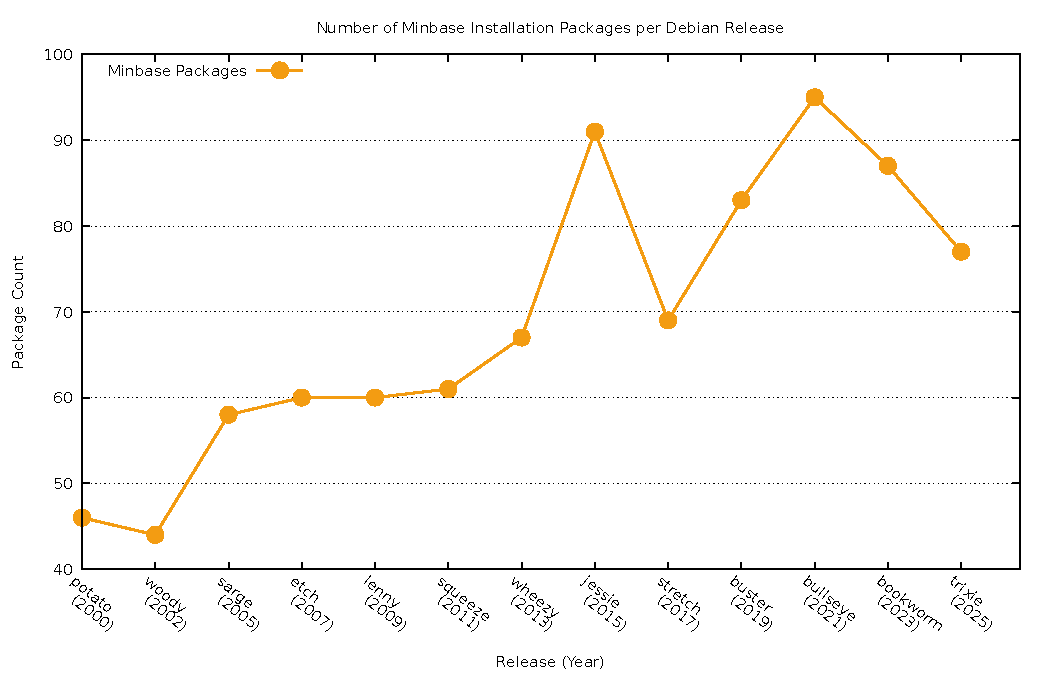
\includegraphics[width=\textwidth]{package_count.pdf}
  \caption[Minbase package count per release.]{Number of binary packages resolved by \texttt{debootstrap -{}-variant=minbase} for each stable release from Potato (2000) to Trixie (2025). The vertical axis gives the package count and each point is one release. The series is computed over the whole minbase population rather than the persistent subset.}
  \label{fig:package-count}
\end{figure}

The swing from Wheezy (67) to Jessie (91) and on to Stretch (69) amounts to a rise of 24 packages to the local peak followed by a fall of 22. \autoref{fig:init-transition} decomposes the minbase of these three releases by set membership. A core of 53 binary packages is common to Wheezy and Stretch and is present throughout the window. In addition to this common core, Wheezy carries 14 packages that Stretch no longer includes; Jessie carries 10 of those legacy packages that it still shares with Wheezy, 11 newly arrived packages that persist into Stretch, and 17 that appear in Jessie alone ($53 + 10 + 11 + 17 = 91$); and Stretch carries 16 packages absent from Wheezy. The height of the Jessie bar is therefore produced not by any single new component but by the simultaneous presence of legacy packages, newly arrived packages, and a transient set unique to that release.

\begin{figure}[ht]
  \centering
  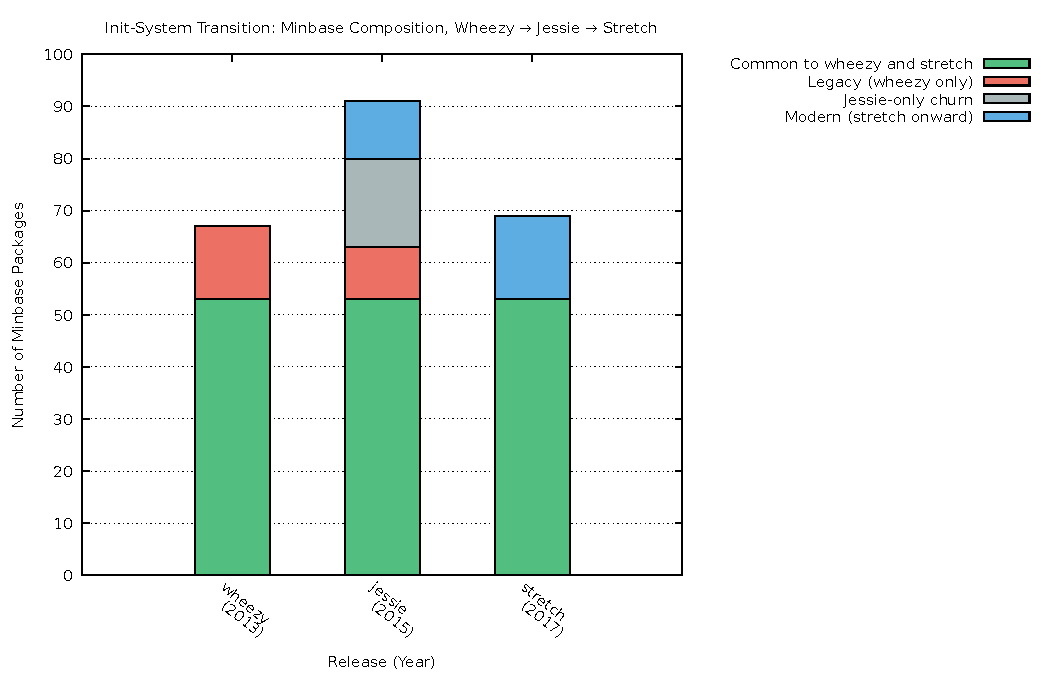
\includegraphics[width=\textwidth]{init_transition.pdf}
  \caption[Minbase composition across the init-system transition.]{Set-membership decomposition of the minbase binary-package list for Wheezy (2013), Jessie (2015), and Stretch (2017), drawn as stacked bars. The vertical axis counts binary packages. Each bar is partitioned into packages common to Wheezy and Stretch, legacy packages present in Wheezy but not Stretch, packages present only in Jessie, and modern packages present from Stretch onward.}
  \label{fig:init-transition}
\end{figure}

This composition coincides with Debian's transition to \texttt{systemd} as the default init system, which took effect in Jessie~\cite{debianJessieReleaseNotes}. The \texttt{systemd} runtime stack entered the required set in Jessie, drawing in \texttt{udev}, which had been merged into \texttt{systemd} upstream~\cite{lwnUdevSystemd} and is built from the \texttt{systemd} source package from Stretch onward~\cite{pkgUdevStretch}, alongside device-management and capability-handling helpers. In Jessie the legacy \texttt{sysvinit} scaffolding (\texttt{initscripts}, \texttt{insserv}, \texttt{sysv-rc}) was still present alongside this new stack and constitutes the legacy band, while the \texttt{systemd} and \texttt{udev} binaries themselves, together with their device-mapper and cryptsetup helpers, make up most of the transient Jessie-only set. By Stretch the legacy scaffolding had been removed and the \texttt{systemd} binary itself had left the chroot-oriented minbase, leaving only the shared libraries that constitute the modern band from Stretch onward. The reduction is consistent with the project's ongoing effort to shrink the \texttt{Essential} and \texttt{Priority: required} sets~\cite{debianEssentialOnDiet,bts851747}, an effort that periodic priority-requalification reviews carry out across release cycles~\cite{debianBusterRequalification}.

The later decline from the Bullseye maximum of 95 packages through 87 in Bookworm to 77 in Trixie is, like the Jessie movements, a composition effect rather than a contraction of the base system. Comparing the minbase sets of these releases attributes the decline to four packaging mechanisms. First, library soname and version bumps, changes to the versioned identity that a shared library exposes to its consumers, which require a correspondingly renamed binary package, retire an old runtime package as its successor arrives: the per-release \texttt{gcc-N-base} packages are replaced each cycle, \texttt{libffi7} gives way to \texttt{libffi8}, \texttt{libsemanage1} and \texttt{libsepol1} to their version-2 successors, and \texttt{libapt-pkg6.0} to \texttt{libapt-pkg7.0}. Second, the Trixie cycle carried out the project-wide 64-bit \texttt{time\_t} transition~\cite{debianTrixieReleaseNotes,debian64bitTime}, which widened the C type that represents calendar time from 32 to 64 bits to avert its overflow in 2038; because this alters the binary interface of every library that exposes the type, many libraries were rebuilt under new binary-package names carrying a \texttt{t64} suffix, so that \texttt{libnettle8} became \texttt{libnettle8t64} and \texttt{libdb5.3} became \texttt{libdb5.3t64}; these are renames of the same code rather than additions or removals. Third, several dependency chains left the required set as the packages that pulled them in were removed or replaced: the Sun RPC and NIS libraries (\texttt{libtirpc3}, \texttt{libnsl2}) and the Kerberos libraries they depended on left the required set between Bullseye and Bookworm, and between Bookworm and Trixie Debian's archive-signature verification moved from \texttt{gpgv} to the Sequoia tool \texttt{sqv}~\cite{aptSequoia}, with much of the surrounding GnuTLS and Nettle chain leaving the minbase alongside these changes.

A smaller part of the decline is the requalification of what a minimal chroot needs rather than a library rename. The filesystem tools \texttt{e2fsprogs} and their libraries, the account-management tool \texttt{adduser}, and the LSB init-script helper \texttt{lsb-base}, which Bookworm reduces to an empty transitional package~\cite{lsbBaseObsolete}, all leave the required set across these releases; a chroot or container image creates no filesystems and manages no interactive accounts, so none of these is needed to populate it. The departure of \texttt{e2fsprogs} is also why the persistent subset present in Trixie's minbase numbers 24 rather than 25 source packages. Working in the opposite direction, the same window adds binary packages that carry no new code: \texttt{util-linux} was split so that \texttt{util-linux-extra} became a separate binary package in Bookworm, and the merged-\texttt{/usr} transition, the consolidation of \texttt{/bin}, \texttt{/sbin}, and \texttt{/lib} into their counterparts under \texttt{/usr} with compatibility symlinks, required from Bookworm~\cite{debianUsrMerge}, added the marker package \texttt{usr-is-merged}. These offsetting renames, splits, and requalifications are precisely why the package count is a weak indicator of size: across Bullseye to Trixie the count falls by 18 packages, yet over the same window the installed size of the persistent core (\autoref{fig:installed-size}) holds near 82~MB and its lines of code (\autoref{fig:nloc}) continue to rise. The recent decline therefore reflects packaging structure, not a reduction in the base system's code or capability.

\section{Installed Size}
\label{sec:results-size}

\autoref{fig:installed-size} reports the installed footprint of the minbase installation and of its persistent subset across the 13 releases. The full minbase grows from approximately 28~MB in Potato to a maximum of approximately 122~MB in Bullseye, ending at approximately 117~MB in Trixie, an increase of roughly fourfold. The persistent subset grows in parallel from approximately 20~MB to approximately 82~MB. The shaded band between the two lines is the footprint contributed by transient packages that belong to the current minbase but not to the long-lived core.

\begin{figure}[ht]
  \centering
  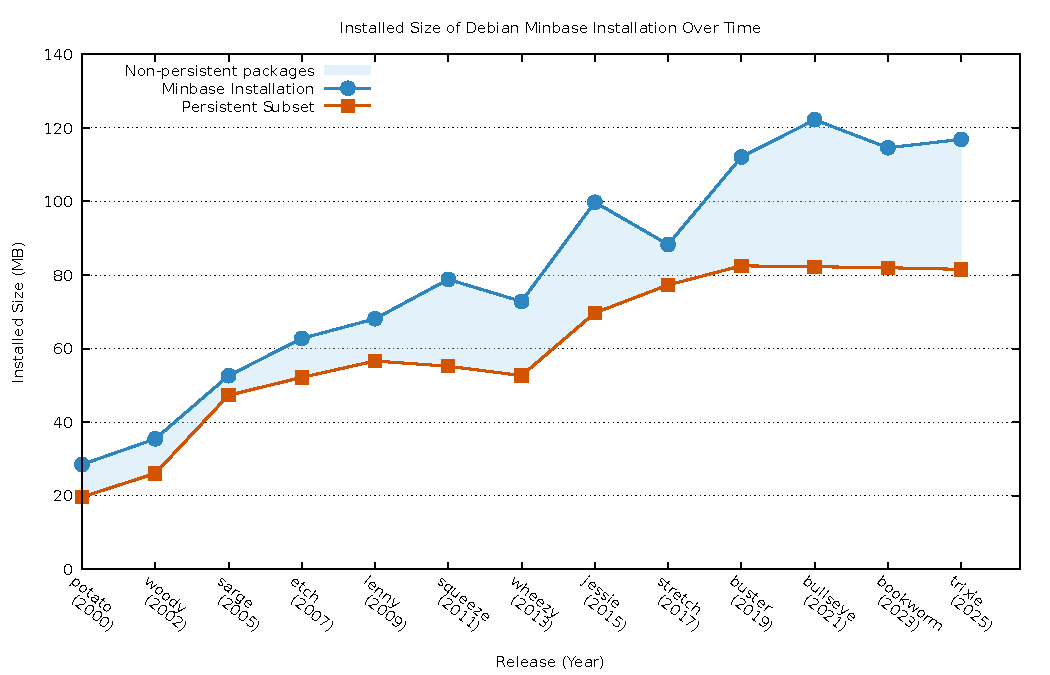
\includegraphics[width=\textwidth]{installed_size.pdf}
  \caption[Installed size of the minbase installation and its persistent subset.]{Installed size in megabytes of the full minbase installation (upper line) and of its persistent subset (lower line) for each stable release from Potato to Trixie, computed from the \texttt{Installed-Size} field of the \texttt{Packages} index. The shaded band between the two lines is the footprint of the transient (non-persistent) packages. Both series are measured over the \texttt{-{}-variant=minbase} tier and differ only in which packages are summed.}
  \label{fig:installed-size}
\end{figure}

Two features of the figure correspond to the composition analysis above. The step from Wheezy (approximately 73~MB) to Jessie (approximately 100~MB) in the minbase line is the largest single increase on the chart, and it coincides with the sharp rise in package count at Jessie and the init-system transition that produced it. The persistent line, by contrast, rises more smoothly and reaches an approximately 82~MB plateau from Buster onward, remaining nearly flat across Buster, Bullseye, Bookworm, and Trixie. Because the persistent subset measures a near-fixed population of long-lived packages, its flattening indicates that the footprint of the core has stabilised in recent releases, while the minbase line continues to oscillate as the surrounding transient set changes. The gap between the two lines, the transient footprint, widens to approximately 30 to 40~MB in the most recent releases: the transient set accounts for a growing share of the minbase total while the persistent core holds near its 82~MB plateau.

\section{Dependency Structure}
\label{sec:results-deps}

The dependency dimension is computed over the whole minbase rather than the persistent subset, because inter-package coupling is a property of the installation as a whole and the arrival of new hub packages, which the fixed persistent core would not capture, is the coupling change this dimension is designed to detect. \autoref{fig:dependency-distribution} shows the per-release distribution of the number of dependencies each package declares. The centre of the distribution is stable: the median is one dependency per package in every release after Potato, the interquartile range spans zero to two in most releases, and the upper whisker ranges from two to five across releases. The typical minbase package has therefore declared between zero and two dependencies for the full 25-year span, and neither the central tendency nor the spread has shifted.

\begin{figure}[ht]
  \centering
  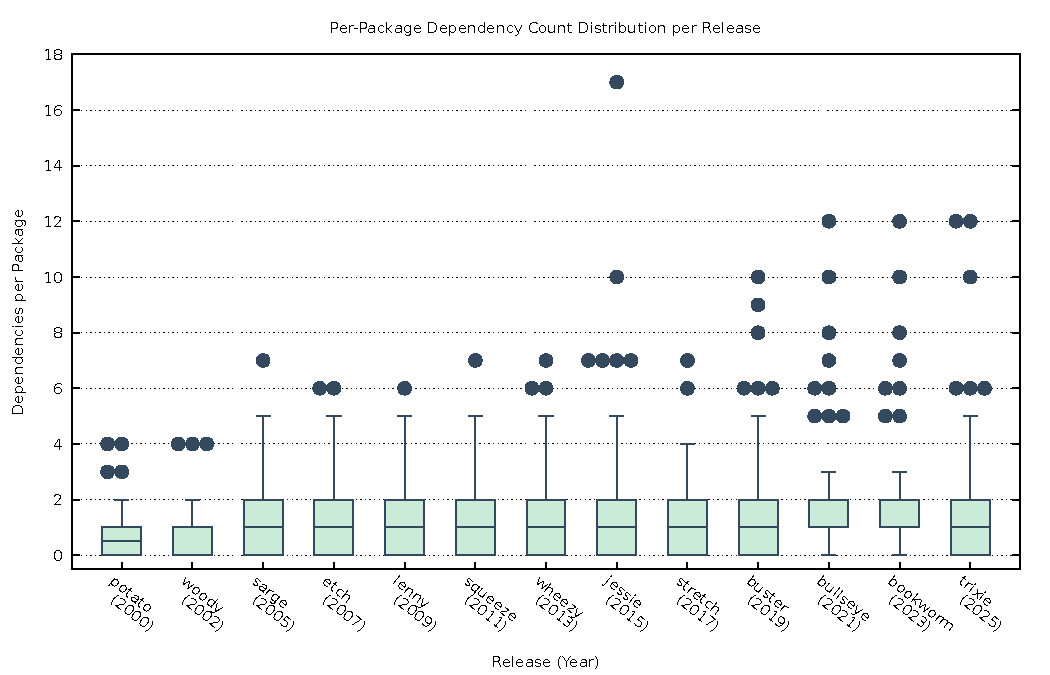
\includegraphics[width=\textwidth]{dependency_distribution.pdf}
  \caption[Distribution of per-package dependency counts per release.]{Per-release distribution of the number of entries each package declares in its \texttt{Depends} field, over the whole minbase installation, from Potato to Trixie. Boxes span the interquartile range (Q1 to Q3), the line inside each box is the median, whiskers extend to the most distant point within $1.5\times$ the interquartile range, and filled circles are outliers beyond the whiskers. Alternatives of the form \texttt{a | b} count as a single edge.}
  \label{fig:dependency-distribution}
\end{figure}

The only quantity that moves is the upper tail of outliers. The maximum dependency count grows from 4 in Potato and Woody, through 6 to 7 in the middle releases, to a single outlier of 17 in Jessie, the highest value in the dataset, before settling at 10 to 12 from Buster onward. The package responsible for this outlier is \texttt{systemd} itself, whose binary package declares 17 dependencies in Jessie. Nine of these are the shared libraries that the \texttt{systemd} binaries link against, among them \texttt{libcap2}, \texttt{libselinux1}, \texttt{libcryptsetup4}, \texttt{libkmod2}, \texttt{libaudit1}, and \texttt{libpam0g}; the remainder are runtime and setup helpers together with the \texttt{sysvinit}-compatibility packages \texttt{initscripts} and \texttt{sysv-rc} and the device manager \texttt{udev}, all drawn into the required set when \texttt{systemd} becomes the default init system (\autoref{sec:composition}). The outlier is therefore the dependency-side signature of the same structural event visible in the package-count and installed-size figures. The dependency dimension thus indicates that increasing coupling in the minbase is concentrated in a small number of hub packages arriving over time, while the rest of the minbase remains as loosely coupled as it was in 2000.

\section{Lines of Code}
\label{sec:results-loc}

\begin{figure}[ht]
  \centering
  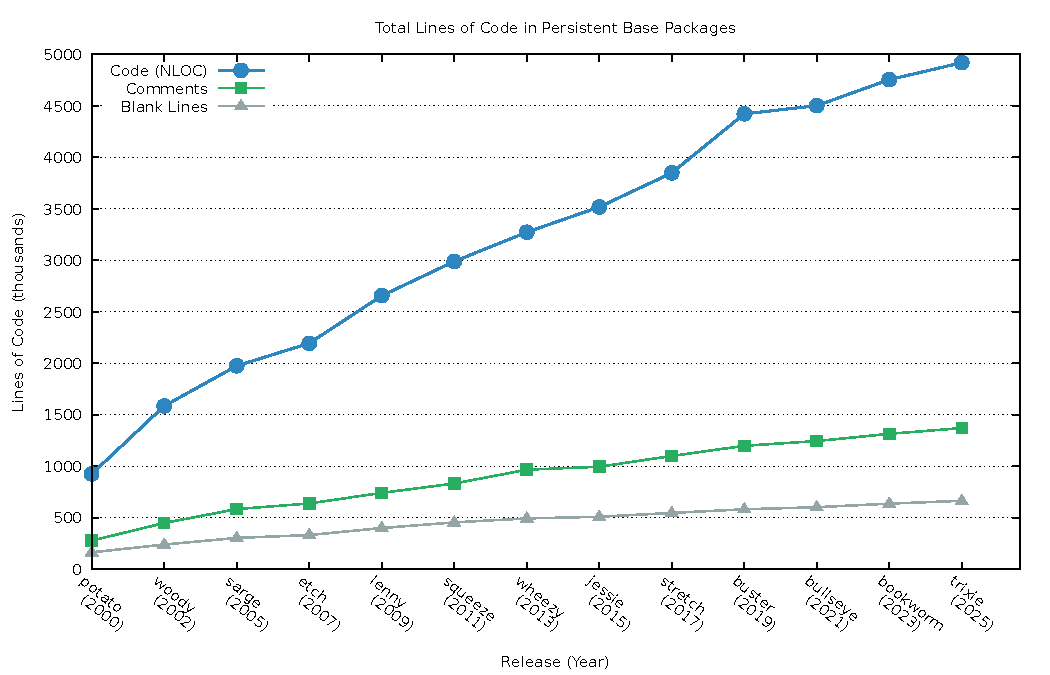
\includegraphics[width=\textwidth]{nloc.pdf}
  \caption[Lines of code, comments, and blank lines in the persistent core.]{Total lines of code, comment lines, and blank lines across the upstream source of the persistent packages, measured with \texttt{tokei}, for each stable release from Potato to Trixie. The vertical axis is in thousands of lines. The counts reflect the upstream source tarballs only and do not include Debian's patches.}
  \label{fig:nloc}
\end{figure}

The lines-of-code dimension is presented through three figures that decompose the same total along different axes: by line type, by package, and by programming language. \autoref{fig:nloc} reports the aggregate total. The total lines of code across the upstream source of the persistent packages grow from approximately 0.92~million in Potato to approximately 4.92~million in Trixie, an increase of roughly 5.3-fold for a population that is fixed by construction. The growth is smooth and monotonic: every release is larger than its predecessor, with no step changes or plateaus. The proportions of code, comment, and blank lines remain stable at roughly 70, 20, and 10 percent throughout, which indicates that commenting density did not erode as the corpus grew fivefold. These counts reflect the upstream source tarballs only and do not include Debian's own modifications, which are treated separately in \autoref{sec:results-patch}. The sustained growth of a fixed set of long-lived packages is consistent with the continuing-growth tendency that Lehman~\cite{Lehman1980Laws} and Wirth~\cite{Wirth1995Plea} describe.

\begin{figure}[ht]
  \centering
  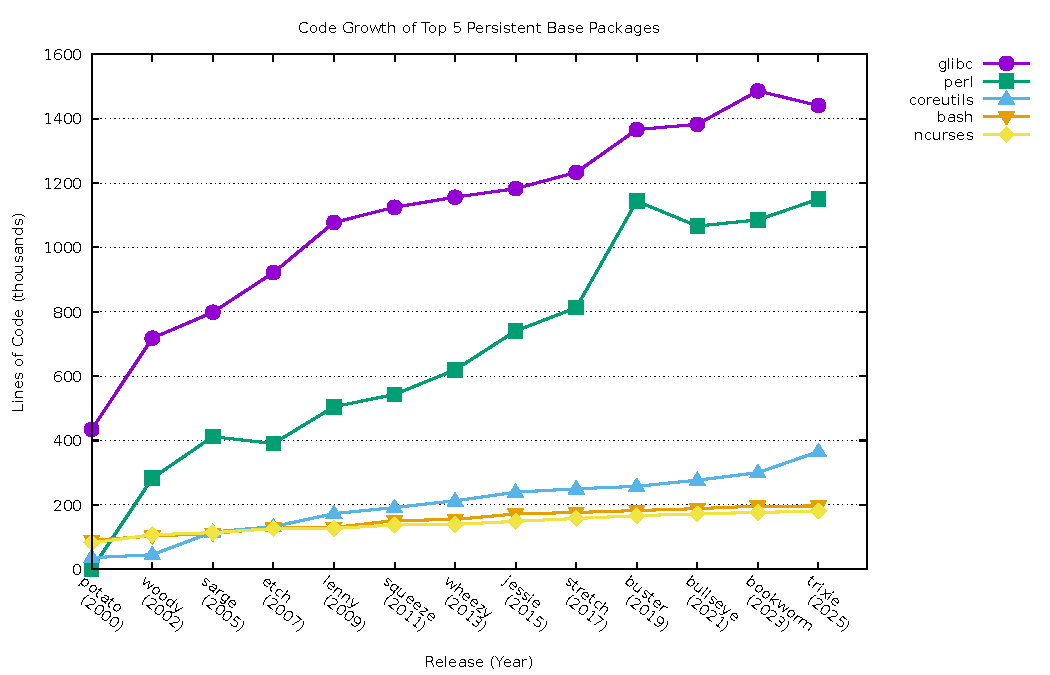
\includegraphics[width=\textwidth]{persistent_growth.pdf}
  \caption[Code growth of the five largest persistent packages.]{Lines of code for the five persistent source packages with the largest total code volume (\texttt{glibc}, \texttt{perl}, \texttt{coreutils}, \texttt{bash}, and \texttt{ncurses}), measured with \texttt{tokei} across the stable releases from Potato to Trixie. Each curve traces one source package and the vertical axis is in thousands of lines. The \texttt{perl} curve reads zero in Potato.}
  \label{fig:persistent-growth}
\end{figure}

\autoref{fig:persistent-growth} attributes this aggregate to individual packages by tracing the five persistent source packages with the largest total code volume. \texttt{glibc} is the largest package in every release, growing from approximately 434{,}000 lines in Potato to approximately 1.44~million in Trixie. \texttt{perl}, which is absent from Potato's minbase and therefore reads zero there, enters at approximately 283{,}000 lines in Woody and grows to approximately 1.15~million, approaching \texttt{glibc} in total line count from Buster onward. \texttt{coreutils} shows the largest relative growth of the five, expanding roughly tenfold from approximately 36{,}000 to approximately 365{,}000 lines, while \texttt{bash} and \texttt{ncurses} grow more modestly, each roughly doubling to approximately 196{,}000 and 181{,}000 lines respectively. Unlike the early pipeline run reproduced in \autoref{fig:nloc-artefact}, which exhibited measurement artefacts, every curve here grows smoothly and without zero-valued gaps, confirming that the artefacts were resolved.

\begin{figure}[ht]
  \centering
  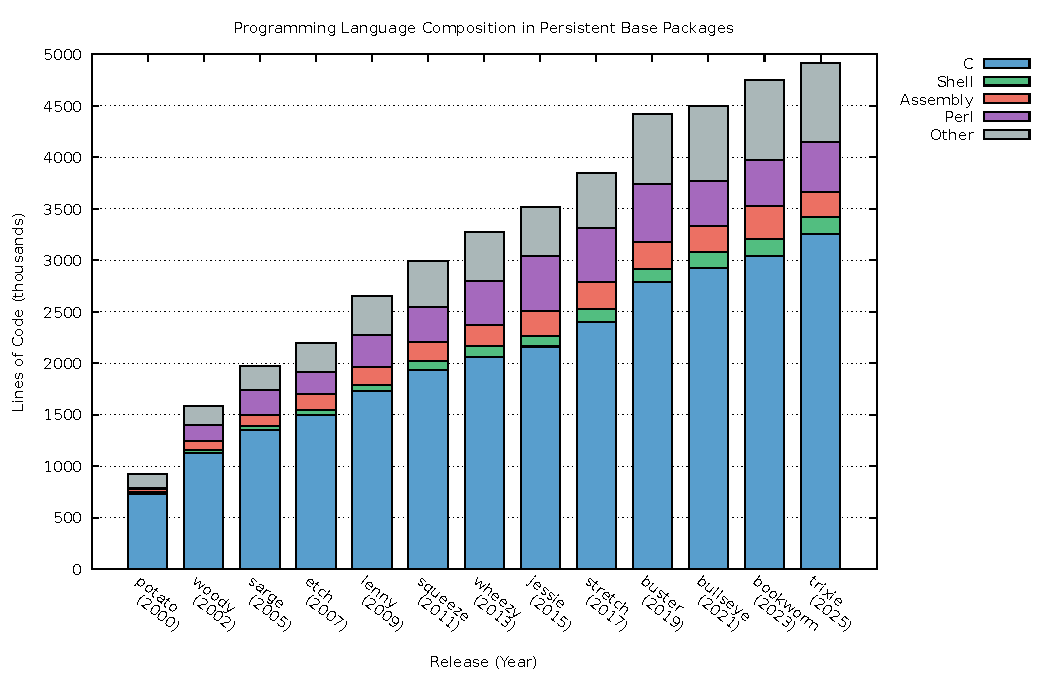
\includegraphics[width=\textwidth]{language_breakdown.pdf}
  \caption[Programming-language composition of the persistent core.]{Lines of code in the upstream source of the persistent packages, decomposed by programming language and stacked per release, measured with \texttt{tokei}, from Potato to Trixie. The vertical axis is in thousands of lines. The \texttt{Other} band collects translation files, documentation, build-system data, and configuration, and also absorbs Python.}
  \label{fig:language-breakdown}
\end{figure}

\autoref{fig:language-breakdown} decomposes the same total by programming language. C is the largest single language in every release, growing from approximately 730{,}000 lines in Potato to approximately 3.25~million in Trixie. Measured by share of the total, however, C declines from approximately 79 percent to approximately 66 percent across the same span, because it grows more slowly than the corpus as a whole. The decline in C's share is offset chiefly by the growth of \texttt{perl}, which rises from roughly 1 percent of the total to roughly 10 percent as the \texttt{perl} package enters and grows. The remaining categories are comparatively stable in share: the \texttt{Other} band, which collects translation files, documentation, build-system data, and configuration, holds between roughly 12 and 16 percent, Assembly between roughly 4 and 7 percent, and Shell between roughly 2 and 3.5 percent. Python remains below 0.4 percent of the total in every release and is grouped into the \texttt{Other} band for that reason. No language displaces C from its dominant position, and no newer systems language, such as Rust, appears in the persistent core within the window. Because C alone accounts for at least three-fifths of the corpus in every release, the complexity analysis in the following section covers the majority of the core.

\section{Per-Function Cyclomatic Complexity}
\label{sec:results-cc}

The complexity dimension is reported at two levels: the central tendency of the per-function complexity, and the shape of its distribution. \autoref{fig:complexity} plots the mean and median modified cyclomatic complexity per function across the C and C++ source of the persistent packages. The number of functions analysed grows from approximately 15{,}900 in Potato to approximately 55{,}000 in Trixie. The mean complexity per function rises by 0.29, from 6.29 in Potato to a peak of 6.58 in Jessie, and then declines to 6.08 in Trixie. The median is flat at exactly 3 in every one of the 13 releases. The typical function in the persistent core has therefore had a cyclomatic complexity of 3 for 25 years, even as the number of functions more than tripled.

\begin{figure}[ht]
  \centering
  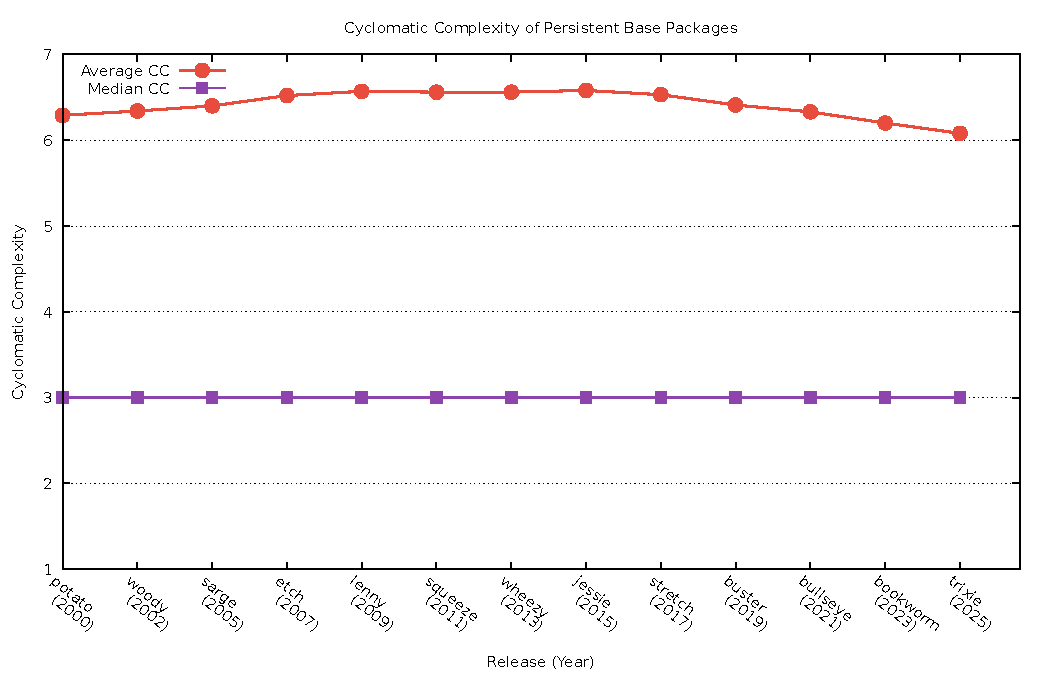
\includegraphics[width=\textwidth]{complexity.pdf}
  \caption[Mean and median per-function cyclomatic complexity per release.]{Average (mean) and median modified cyclomatic complexity per function across the C and C++ source of the persistent packages, measured with \texttt{pmccabe}, for each stable release from Potato to Trixie. Each point aggregates all functions measured in that release. The vertical axis is cyclomatic complexity.}
  \label{fig:complexity}
\end{figure}

\autoref{fig:cc-distribution} shows the per-release distribution behind these summary statistics. The boxes are nearly identical across the 13 releases: the first quartile sits at 1, the median at 3, and the third quartile at 7, narrowing slightly to 6 in Bookworm and Trixie. The interquartile range is thus stable across the full period, contracting slightly in the two most recent releases. The distribution has a long right tail, and the outliers beyond the whiskers are suppressed in the figure for legibility. The maximum complexity, reported here rather than plotted, grows from 273 in Potato to 1{,}125 in Jessie and stands at 1{,}048 in Trixie. The single most complex function in every release after Potato is the hand-written tokenizer and keyword recogniser of \texttt{perl} (the functions \texttt{Perl\_yylex} and \texttt{Perl\_keyword}); this extreme value is a property of one upstream source file rather than of the core as a whole.

\begin{figure}[ht]
  \centering
  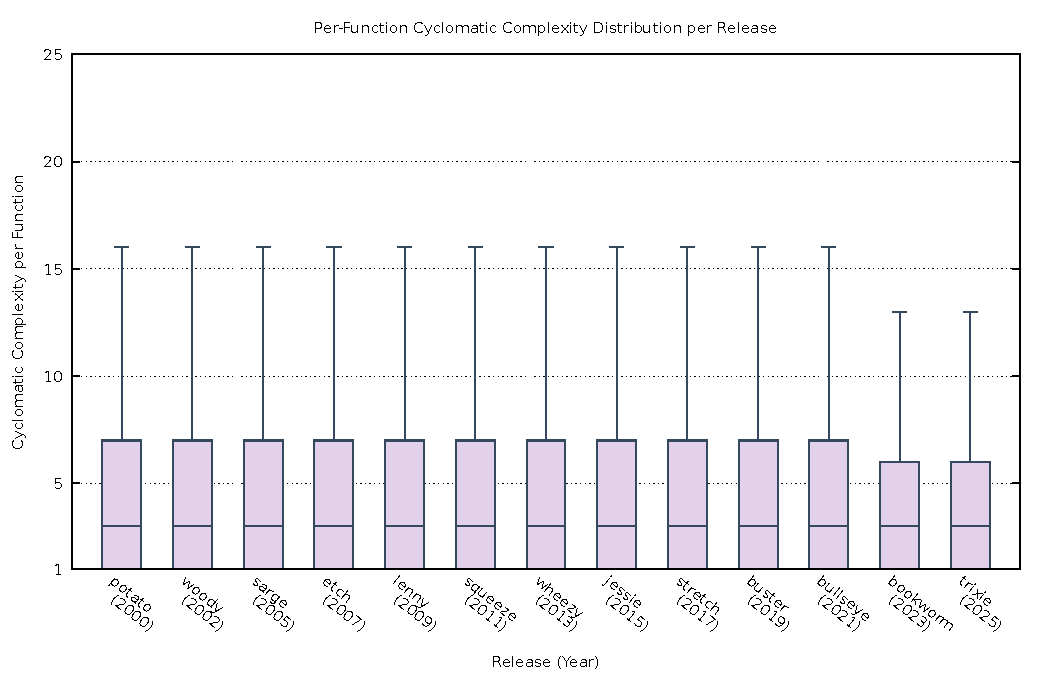
\includegraphics[width=\textwidth]{cc_distribution.pdf}
  \caption[Per-function cyclomatic complexity distribution per release.]{Per-release distribution of modified cyclomatic complexity over all functions in the C and C++ source of the persistent packages, measured with \texttt{pmccabe}, from Potato to Trixie. The vertical axis is complexity per function. Boxes span the interquartile range, the line inside each box is the median, and whiskers extend to the most distant point within $1.5\times$ the interquartile range; outliers beyond the whiskers are suppressed for legibility.}
  \label{fig:cc-distribution}
\end{figure}

The three observations, a function count that more than triples, a median that holds at 3, and a mean that rises gently to a peak before declining, indicate that the growth of the C and C++ core occurs through the addition of many small, low-complexity functions rather than through an increase in the complexity of the typical function. This pattern is consistent with the result that Israeli and Feitelson report for the Linux kernel, where total complexity rises while the average complexity of individual functions falls as new low-complexity functions are added~\cite{israeli2010linux}. The observation is reported here as a description of the measured trend and not as a causal claim. As noted in \autoref{sec:metric-cc}, the complexity measurement covers only the C and C++ source and therefore describes 23 of the 25 persistent packages; its scope is revisited in \autoref{sec:limitations}.

\section{Distribution-Specific Patch Volume}
\label{sec:results-patch}

The final dimension is the volume of distribution-specific patches that Debian applies to the persistent packages. As established in \autoref{sec:patch-inconsistency}, this metric is not comparable across the change in Debian's source-package format: counts produced under the \texttt{1.0} (\texttt{.diff.gz}) format are inflated by non-code material bundled into the single diff, whereas the \texttt{3.0 (quilt)} format from Jessie onward records only named patches. \autoref{fig:patch-size} reflects this by drawing the \texttt{1.0}-era releases in grey for context, marking the format boundary, and drawing the comparable \texttt{3.0 (quilt)} era in solid colour. Within the grey era the series is volatile and peaks at approximately 904{,}000 lines in Wheezy, but these values are dominated by packaging artefacts rather than by code changes and are not interpreted.

\begin{figure}[ht]
  \centering
  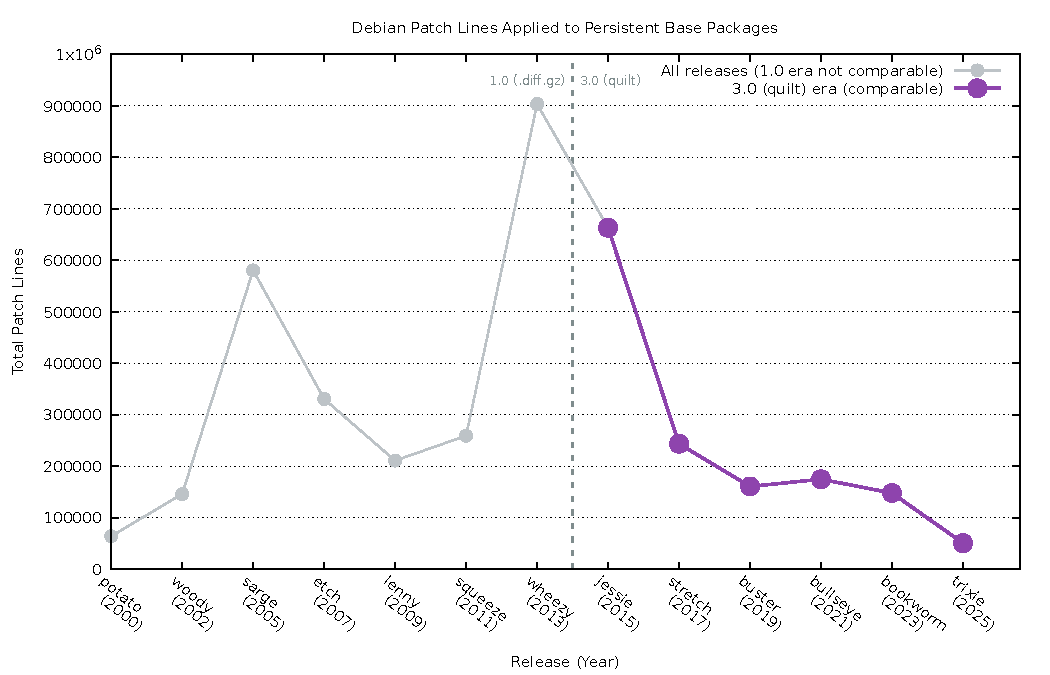
\includegraphics[width=\textwidth]{patch_size.pdf}
  \caption[Debian patch lines applied to the persistent core per release.]{Total number of Debian patch lines across the persistent packages for each stable release from Potato to Trixie. The vertical axis counts patch lines. Releases packaged under the \texttt{1.0} (\texttt{.diff.gz}) source format are drawn in grey and those under the \texttt{3.0 (quilt)} format from Jessie onward in solid colour, with the format boundary marked. The counts are comparable only within the \texttt{3.0 (quilt)} era.}
  \label{fig:patch-size}
\end{figure}

Within the comparable \texttt{3.0 (quilt)} era, the total patch volume across the persistent core declines from approximately 663{,}000 lines in Jessie to approximately 51{,}000 in Trixie. The \texttt{glibc} package is the dominant contributor in every release, accounting for approximately 570{,}000 of the Jessie total and approximately 37{,}000 of the Trixie total. The declining trend suggests that the named patch set Debian maintains against the persistent core has contracted over the most recent releases, although the metric counts patch lines, including diff context, rather than the number of semantic changes, so it should be read as an indicator of patch bulk rather than of maintenance effort.

The secondary research question also asks about the file-level structure of these patches. The structure changes sharply at the format transition: under the \texttt{1.0} format a package's Debian-specific material is carried in a single \texttt{.diff.gz} file, while native packages such as \texttt{dpkg}, whose upstream is the Debian project itself and which therefore ship no separate patch archive, carry none, whereas under \texttt{3.0 (quilt)} the same material is split into many named patch files under \texttt{debian/patches/}. The transition occurs at different releases for different packages, around the Jessie to Stretch window, and several persistent packages had already migrated to the quilt format by Squeeze and Wheezy; \texttt{glibc}, for instance, moves from a single diff to 281 named patches at Jessie, while \texttt{coreutils} retains a single file until Stretch. This shift from one bundled diff to many purpose-specific patches following the DEP-3 tagging convention~\cite{dep3} is the file-level structural evolution the secondary question identifies, and it is also what confines the post-Jessie counts to Debian's code-level modifications.


\chapter{Discussion}\label{ch:discussion}
The results chapter reported each of the five dimensions as an independent release-wise series. This chapter draws those series together in answer to the research questions, relates the synthesis to the prior work reviewed in \autoref{ch:relatedwork}, states the limitations that bound the findings, and identifies directions for future work. Consistent with the exploratory-descriptive framing established in \autoref{ch:introduction}, the synthesis below characterises and situates what was measured; it does not assert a causal or correlational relationship between the dimensions, and the inferential analysis that such claims would require remains a direction for future work.

\section{Principal Findings}
\label{sec:principal-findings}

The central observation that the primary research question yields is a divergence between the size of the persistent core and the complexity of its constituent parts. Over the 25 years from Potato to Trixie, the persistent core grew by roughly 5.3-fold in lines of code, from approximately 0.92 to approximately 4.92 million (\autoref{fig:nloc}), and its installed footprint grew roughly fourfold, from approximately 20 to approximately 82~MB (\autoref{fig:installed-size}), for a population that is fixed by construction. Across the same span, however, the per-function cyclomatic complexity did not rise: the median held at exactly 3 in every one of the 13 releases, and the mean rose by only 0.29 to a peak of 6.58 at Jessie before declining to 6.08 at Trixie, a value below its starting point of 6.29 (\autoref{fig:complexity}). The per-package dependency count was similarly stationary, with a median of one edge per package in every release after Potato (\autoref{fig:dependency-distribution}). The descriptive picture is therefore one of growth by accretion: as the number of analysed functions more than tripled, from approximately 15{,}900 to approximately 55{,}000, the core expanded through the addition of many small, low-complexity, loosely coupled units rather than through an increase in the complexity or coupling of the typical unit. The fifth dimension that the primary question names, distribution-specific patch volume, is synthesised below together with the secondary research question that sharpens it.

The secondary research question on composition is answered by a non-monotonic package count whose movements are attributable to packaging structure rather than to changes in capability. The minbase count rises and falls between 44 and 95 packages across the releases (\autoref{fig:package-count}), and the two largest movements both resolve into composition effects on inspection: the peak at Jessie is produced by the simultaneous presence of legacy, newly arrived, and transient packages during the \texttt{systemd} init-system transition (\autoref{fig:init-transition}), and the subsequent decline is produced by library soname bumps, the 64-bit \texttt{time\_t} rebuild, the departure of dependency chains, and the requalification of what a minimal chroot requires. Because splitting and renaming packages move the count without adding or removing code, the count is a weak indicator of size; the installed-size and lines-of-code dimensions are the stronger signals. Those stronger signals indicate that recent growth is carried by the transient set rather than by the long-lived core: the persistent footprint plateaus near 82~MB from Buster onward while the gap to the full minbase widens to approximately 30 to 40~MB.

The secondary research question on distribution-specific patches is answered only within the window in which the metric is comparable. As established in \autoref{sec:patch-inconsistency}, patch-line counts under the \texttt{1.0} source format are inflated by non-code material bundled into a single diff, so the series is interpreted only from Jessie onward under the \texttt{3.0 (quilt)} format. Within that window the total patch volume across the persistent core declines from approximately 663{,}000 to approximately 51{,}000 lines (\autoref{fig:patch-size}), a total dominated in every release by \texttt{glibc}, which alone accounts for approximately 570{,}000 of the Jessie figure and approximately 37{,}000 of the Trixie figure. The file-level structure changed in parallel, from a single bundled \texttt{.diff.gz} to many named patches under the DEP-3 convention~\cite{dep3}; \texttt{glibc}, for instance, moves from one diff to 281 named patches at Jessie. The decline therefore describes a contraction in the bulk of Debian's named modifications to the persistent core, though, because the metric counts patch lines including diff context rather than semantic changes, it indicates the bulk of the distribution's modifications rather than the effort required to produce them.

One structural event recurs across these dimensions. The arrival of \texttt{systemd} in the required set at Jessie is visible simultaneously as the peak in package count, the largest single step in the minbase installed-size series, and the single dependency outlier of 17 edges that is the highest value in the dataset. This co-visibility is a descriptive coincidence: a single packaging decision left a trace in three metrics computed independently from the same release. It does not show that any one dimension drives another, a claim the descriptive design of this thesis cannot establish.

\section{Relation to Prior Work}
\label{sec:relation-prior-work}

The continuing growth of the persistent core is a direct instance of the tendency that Lehman formalised and that Wirth restated. Lehman's laws hold that actively used software continually grows unless effort is invested otherwise~\cite{Lehman1980Laws}, and Wirth argued that this growth had become a structural problem in which resource demands outpaced functional gains~\cite{Wirth1995Plea}. The 5.3-fold growth in lines of code of a fixed package population, observed here for a minimal base system rather than for an application, is consistent with both accounts. The companion proposition that complexity increases unless deliberately countered holds in the present data only at the aggregate level: the total complexity summed over all functions rises with the function count, and the maximum per-function complexity grows from 273 to a peak of 1{,}125 (\autoref{sec:results-cc}), yet the complexity of the typical function does not increase. The data therefore supports the continuing-growth tendency while qualifying the increasing-complexity tendency at the granularity of the individual function.

A particularly close correspondence is with the kernel study of Israeli and Feitelson. They reported that the total complexity of the Linux kernel rises over time while the average complexity of individual functions falls, because new code is introduced as many small, low-complexity functions~\cite{israeli2010linux}. The persistent Debian core reproduces this mechanism on a different corpus: the function count triples, the median per-function complexity is stationary, and the mean declines after its Jessie peak. The agreement extends their kernel-specific observation to the base of a complete distribution and supports their methodological argument that total and average complexity must be reported together, because either measure in isolation would misrepresent the trend.

The growth-rate studies of the kernel admit a more guarded comparison. Godfrey and Tu reported super-linear growth in kernel lines of code~\cite{godfrey2000linux}, and Koren contrasted the faster accumulation of code in development branches against stable ones~\cite{koren2006linux}. The persistent core analysed here grows smoothly and monotonically, but over a package population that is fixed by construction, so its trajectory measures within-package growth and excludes the arrival of new modules that drives super-linear whole-system curves. The present design isolates a different component of growth rather than contradicting these results. At the broader level of empirical validation, Neamtiu et al.\ and Vasa each found continuing growth and continuing change to be the most robustly confirmed of Lehman's laws across many individual projects~\cite{neamtiu2009towards,vasa2010growth}; the present work adds an observation of the same tendency at the granularity of a whole distribution's base.

The dependency findings relate to the network studies of the Debian ecosystem. LaBelle and Wallingford, De Sousa et al., and Horváth each characterised Debian's inter-package dependency graph as scale-free, with new edges accumulating by preferential attachment~\cite{interPackageDependency,sousa2009debian,horvath2012linuxdeps}. The present result, in which the median package has declared between zero and two dependencies for the full 25-year span while all movement is confined to a small number of hub packages such as \texttt{systemd}, is consistent with a hub-dominated structure of that kind. The agreement is suggestive rather than a replication, because the measurement here covers only the small minbase subgraph rather than the full archive of more than eighteen thousand packages that those studies analysed.

The patch-volume dimension connects to the literature on distribution-level maintenance. Becker et al.\ analysed Debian maintainer scripts at scale with the CoLiS platform~\cite{becker2022colis}, and Lin et al.\ quantified the share of fixes contributed locally by distribution maintainers rather than propagated from upstream~\cite{lin2022upstream,lin2023vulnerability}. The contraction of the named patch set in the quilt era describes one facet of this maintenance work for the persistent core. The metric here counts patch lines including diff context rather than semantic changes, however, and CoLiS examined maintainer scripts rather than source patches, so the present result complements these studies on a distinct artefact without measuring maintenance effort directly. Molnar and Motogna observed that distribution-level metric trends can diverge from the trends of individual projects~\cite{molnar2020longitudinal}; the present aggregates echo this, in that they are dominated by single packages, with \texttt{glibc} governing both the installed-size and patch-volume totals and a single \texttt{perl} source file governing the maximum complexity. Ronchieri et al.\ established a cyclomatic-complexity baseline for a large scientific toolkit to characterise its maintainability~\cite{ronchieri2016software}; the per-function values reported here, a median of 3 and a mean near 6, provide a comparable baseline for the base of a general-purpose distribution.

Finally, the findings bear on the motivation set out in the introduction. The association that Nguyen et al.\ reported between rising complexity and increased maintenance cost and defect density~\cite{nguyen2017impact}, together with the emphasis that Sherlock et al.\ place on users being able to read and understand the software they run~\cite{Sherlock2018OpenSS}, framed complexity growth as a concern for a base system of Debian's reach. The stationary per-function complexity observed here is consistent with a core whose individual units did not become locally harder to read or maintain over 25 years, even as the corpus grew fivefold. This observation is consistent with those concerns; it is not a causal claim about maintenance outcomes, which the present data cannot support.

\section{Limitations}
\label{sec:limitations}

Cyclomatic complexity is measured only for C and C++ source, because \texttt{pmccabe} supports no other languages. The complexity results therefore describe the compiled C and C++ core of the base system and do not capture packages written in interpreted languages. The per-release complexity aggregates are consequently computed over 23 of the 25 persistent packages: \texttt{debconf} and \texttt{base-files} contribute to the lines-of-code totals but contain no C or C++ source and are therefore absent from the complexity figures. This restriction does not bias the trend within the C and C++ code, but the complexity findings should not be read as a statement about the complexity of the persistent core in its entirety.

The patch-volume metric carries two further measurement limitations. The first, established in \autoref{sec:patch-inconsistency}, is that counts are comparable only within the \texttt{3.0 (quilt)} era from Jessie onward, because the \texttt{1.0} format bundles changelogs, documentation, and other non-code material into a single diff and so inflates the earlier counts; the metric consequently describes Debian's code-level modifications for fewer than half of the releases studied. The second is that the metric counts physical patch lines, including unchanged context lines, rather than the number of semantic changes a patch makes, so it indicates the bulk of the distribution's modifications and not the effort required to produce or maintain them. The lines-of-code metric shares the character of the first concern: \texttt{tokei} counts physical lines in the upstream tarballs, which include generated code, vendored third-party code, and test suites, and the composition of a tarball can vary between releases independently of the code that the package actually builds.

A construct limitation applies to the use of cyclomatic complexity as a measure of complexity in general. Cyclomatic complexity captures the control-flow structure of individual functions and does not measure inter-procedural coupling, data-flow complexity, architectural complexity, or the cognitive difficulty of reading code. The stationary per-function complexity reported here should therefore be understood as a statement about control-flow structure at the function level, and not as evidence that the core has not become more complex along dimensions the metric does not observe.

Two limitations bound the scope to which the findings generalise. First, the persistent core is defined by survival: only the source packages present in the minbase of at least 11 of the 13 releases from Potato to Trixie qualify. This construction yields a conservative and deliberately stable subset, and the long-lived foundational packages it selects need not be representative of the base system as a whole, still less of a full Debian installation. Second, the minbase variant is a minimal, chroot-oriented installation rather than a desktop or server system, so the trajectories reported here characterise the foundation on which larger installations are built and do not describe the size or complexity that a user-facing system would exhibit. The analysis also covers a single distribution, and the processor architecture on which it is measured changes once within the window: releases up to Lenny are measured on i386 and releases from Squeeze onward on amd64 (\autoref{tab:releases}). The installed-size metric depends on the architecture for which a package is built, so the size series crosses this boundary at Squeeze, whereas the lines-of-code, complexity, and patch metrics are computed from architecture-independent source archives and are unaffected. The restriction to one distribution further means that the observed trends cannot be separated into those specific to Debian and those common to long-lived Linux distributions in general.

A final limitation concerns the provenance of the data. The early releases are reconstructed from the Debian snapshot archive~\cite{debianSnapshot}, whose historical source packages occasionally required repacking, and the diagnosis in \autoref{sec:webapp} showed that defects in the extraction of these archives produced measurement artefacts in early pipeline runs. Although the artefacts identified there were corrected, the oldest releases rest on the least uniform source material, and undetected irregularities in that material would affect the earliest points of each series most.

\section{Future Work}
\label{sec:future-work}

The limitations above indicate the most immediate extensions. Replacing or supplementing \texttt{pmccabe} with complexity tools for interpreted languages would bring \texttt{debconf}, \texttt{base-files}, and the growing \texttt{perl} share of the corpus within the scope of the complexity analysis, closing the gap between the lines-of-code and complexity populations. A semantic analysis of the patch archive, counting the changes a patch makes rather than its lines, would convert the patch-volume indicator into a measure that more closely tracks maintenance effort. It would also remove the dependence on the source-package format that confines the present metric to the quilt era.

A second direction broadens the comparison. Applying the same pipeline to other long-lived distributions, such as the Ubuntu and Arch systems studied by Horváth~\cite{horvath2012linuxdeps} or the Fedora system studied by Lin et al.~\cite{lin2022upstream}, would allow the trends reported here to be separated into those specific to Debian and those common to the ecosystem, and extending the analysis from the minbase variant to the standard and desktop tiers would test whether the accretion pattern observed in the minimal base also holds for larger installations. The pipeline could likewise incorporate the additional per-package metrics considered during scoping, in particular the Maintainability Index~\cite{Coleman1994Using}, alongside measures of coupling and cognitive complexity that the present control-flow metric does not capture.

A third direction takes up the inferential questions that the descriptive design of this thesis deliberately set aside. The co-visibility of the \texttt{systemd} transition across three dimensions, and the divergence between rising size and stationary per-function complexity, are observations that invite the correlational and causal analysis that larger samples and controlled comparisons would support. The per-release artefacts produced here are intended as the baseline for such work, and for the evaluation of automated software de-bloating techniques~\cite{quach2018debloating} against a documented historical record of how the base system has actually grown.


\chapter{Conclusion}\label{ch:conclusion}
This thesis set out to provide a reproducible, release-wise account of how the persistent packages of Debian's minbase installation have developed across the distribution's full stable history, a longitudinal characterisation that the existing literature had not assembled. To that end it built a containerised analysis pipeline and applied it to the 25 source packages of the persistent core, those present in the minbase installation of at least 11 of the 13 stable releases from Potato (2000) to Trixie (2025), extracting five metrics per release: installed size, dependency structure, lines of code, per-function cyclomatic complexity, and distribution-specific patch volume.

The resulting artefacts describe a base system that grew in size while remaining stable in the complexity of its parts. The persistent core grew roughly 5.3-fold in lines of code and roughly fourfold in installed footprint over the 25-year period, yet the median per-function cyclomatic complexity held at 3 in every release and the median per-package dependency count at 1 in every release after Potato. The core therefore expanded through the addition of many small, low-complexity, loosely coupled units rather than through an increase in the complexity of the typical unit. The composition of the minbase changed non-monotonically across releases, and its largest movements, the \texttt{systemd} init-system transition at Jessie and the recent decline in package count, are attributable to packaging structure rather than to changes in capability. The volume of distribution-specific patches, comparable only from the adoption of the \texttt{3.0 (quilt)} source format at Jessie onward, declined across the most recent releases and was dominated in every release by \texttt{glibc}; the file-level structure of those patches changed in parallel, from a single bundled \texttt{.diff.gz} per package to many named, purpose-specific patch files.

Alongside these descriptive results, the thesis delivers the means to reproduce and extend them. The pipeline, built from established open-source tools (\texttt{debootstrap}, \texttt{tokei}, \texttt{pmccabe}, and \texttt{gnuplot}) and orchestrated with Docker and a Makefile, regenerates the full set of per-release CSV files and figures from the Debian archives. An interactive companion application, the Debian Bloat Explorer, reads the same CSV files and supports drill-down into individual packages and releases; it was the instrument through which several measurement artefacts, and the patch-metric inconsistency at the source-format transition, were diagnosed.

The contribution of this work is a descriptive baseline rather than an explanatory account. The artefacts characterise what has happened to Debian's persistent core; they do not establish why, and the design supports no causal or correlational claim relating one dimension to another. Whether the divergence between rising size and stationary per-function complexity reflects a general property of long-lived distributions, and what mechanisms produce it, are questions that the reproducible pipeline and per-release data presented here provide a basis to investigate in future work.


\chapter*{References}
\addcontentsline{toc}{chapter}{References}
\markboth{References}{}
\begingroup
\RaggedRight
% Allow line breaks inside long URLs (e.g. Semantic Scholar paper hashes)
\setcounter{biburlnumpenalty}{9000}
\setcounter{biburllcpenalty}{7000}
\setcounter{biburlucpenalty}{8000}
\printbibliography[heading=none]
\endgroup


\chapter*{Declaration on the Use of AI Tools}
\addcontentsline{toc}{chapter}{Declaration on the Use of AI Tools}
\markboth{Declaration on the Use of AI Tools}{}
During the preparation of this thesis, three AI tools were used as aids. Claude (Anthropic) was used to correct and improve the grammar, wording, sentence structure, and \LaTeX{} syntax of the thesis text. GitHub Copilot (GitHub) was used for code-completion suggestions during the development of the analysis pipeline and the companion application. Consensus, an AI-assisted academic search engine, was used to identify relevant literature and candidate references; the sources identified this way were reviewed before being cited. All output produced by these tools was reviewed and revised by the author. The design of the study, the selection of methods and metrics, the analysis of the data, and the conclusions drawn are the author's own, and the author takes full responsibility for the entire content of this thesis.


\chapter*{Glossary}
\addcontentsline{toc}{chapter}{Glossary}
\markboth{Glossary}{}
\begingroup
\emergencystretch=1.5em
\begin{description}[itemsep=2pt]
    \item[cyclomatic complexity] The number of linearly independent paths through a function's control-flow graph, used as a measure of branching complexity. This thesis reports the modified variant computed by \texttt{pmccabe}, which counts a multi-way \texttt{switch} statement as a single decision point.
    \item[\texttt{debootstrap}] The Debian utility that installs a base system into a target directory without requiring a running Debian host. Its \texttt{-{}-variant=minbase} option resolves the smallest installable package set.
    \item[\texttt{Essential} / \texttt{Priority: required}] Control-field markings in the package index that place a binary package in the mandatory core of every Debian installation; together with their transitive dependencies these packages constitute the minbase set.
    \item[lines of code (NLOC)] The number of physical source lines classified as code, excluding comment and blank lines, counted with \texttt{tokei}.
    \item[merged-\texttt{/usr}] The filesystem layout that consolidates \texttt{/bin}, \texttt{/sbin}, and \texttt{/lib} into their counterparts under \texttt{/usr} with compatibility symlinks; required from Bookworm.
    \item[minbase] The smallest \texttt{debootstrap} installation variant, containing the \texttt{Essential: yes} and \texttt{Priority: required} packages and their transitive dependencies; it carries no kernel or bootloader and targets chroot and container environments.
    \item[native package] A package whose upstream is the Debian project itself, such as \texttt{dpkg}; it has no separate upstream tarball and therefore no distribution-specific patch archive.
    \item[persistent package] A source package whose name, after alias resolution, appears in the minbase set of at least 11 of the 13 releases studied; the 25 packages meeting this criterion form the persistent core.
    \item[snapshot archive] The Debian service at \texttt{snapshot.debian.org} that preserves a timestamped copy of every package version the project has distributed.
    \item[source package / binary package] The source unit from which one or more installable binary packages are built; the \texttt{Source} field of the package index maps each binary package to its source package.
    \item[source-package format] The declared layout of a Debian source package: under \texttt{1.0}, all distribution-specific material is bundled into a single \texttt{.diff.gz}; under \texttt{3.0 (quilt)}, packaging metadata is carried in a \texttt{.debian.tar.*} archive and modifications to upstream source as named patches under \texttt{debian/patches/}.
    \item[transient set] The packages of a release's minbase that do not belong to the persistent core.
\end{description}
\endgroup


\appendix
\chapter{Appendix}\label{english:appendix}
\section{Source Code and Data Availability}
\label{app:availability}

The complete source code of the analysis pipeline and of the Debian Bloat Explorer is publicly available in the thesis repository:
\begin{center}
  \url{https://github.com/hajir3/bachelor-thesis}
\end{center}
The pipeline scripts reside under \texttt{scripts/}, the companion application under \texttt{webapp/}, and the \LaTeX{} source of this document under \texttt{thesis/}. The state of the repository at submission is marked by the git tag \texttt{BA-Submission}; an archival snapshot of this state, including the companion application, is permanently available on Zenodo (DOI: \href{https://doi.org/10.5281/zenodo.20546461}{10.5281/zenodo.20546461}). All figures and per-release values in this thesis derive from a single pipeline run, whose complete CSV files are preserved in the repository under
\begin{center}
  \texttt{output/results/BA-Submission/},
\end{center}
with the corresponding rendered figures under \texttt{output/figures/BA-Submission/}.

A hosted instance of the Debian Bloat Explorer, pinned to the CSV files of this same pipeline run, is publicly available at
\begin{center}
  \url{https://debian-bloat-explorer.streamlit.app}
\end{center}
and requires no local installation.

\clearpage
\section{Per-Release Metric Summary}
\label{app:metrics}

The main chapters of this thesis report rounded values; \autoref{tab:metrics-size} and \autoref{tab:metrics-code} give the exact per-release figures, computed from the CSV files of the pipeline run named in \autoref{app:availability}.

\begin{table}[ht!]
  \centering
  \setkomafont{caption}{\footnotesize}
  \setcapindent{0pt}
  \renewcommand{\arraystretch}{0.95}
  \caption[Per-release composition and installed size of the minbase installation.]{Per-release composition and installed size of the minbase installation, from Potato to Trixie. The packages column counts the binary packages that \texttt{debootstrap -{}-variant=minbase} resolves, the persistent column the number of the 25 persistent source packages present, and the size columns the summed \texttt{Installed-Size} of the minbase and of its persistent subset in megabytes (1~MB = 1024~kB).}
  \label{tab:metrics-size}
  \footnotesize
  \begin{tabular}{llrrrr}
    \hline
    Release & Year & Packages & Persistent & Minbase (MB) & Persistent (MB) \\
    \hline
    Potato   & 2000 & 46 & 20 & 28.5  & 19.6 \\
    Woody    & 2002 & 44 & 21 & 35.4  & 26.1 \\
    Sarge    & 2005 & 58 & 25 & 52.6  & 47.3 \\
    Etch     & 2007 & 60 & 25 & 62.8  & 52.2 \\
    Lenny    & 2009 & 60 & 25 & 68.1  & 56.6 \\
    Squeeze  & 2011 & 61 & 24 & 78.8  & 55.2 \\
    Wheezy   & 2013 & 67 & 24 & 72.8  & 52.7 \\
    Jessie   & 2015 & 91 & 25 & 99.8  & 69.7 \\
    Stretch  & 2017 & 69 & 25 & 88.3  & 77.3 \\
    Buster   & 2019 & 83 & 25 & 112.1 & 82.5 \\
    Bullseye & 2021 & 95 & 25 & 122.2 & 82.3 \\
    Bookworm & 2023 & 87 & 25 & 114.6 & 82.0 \\
    Trixie   & 2025 & 77 & 24 & 116.9 & 81.5 \\
    \hline
  \end{tabular}
\end{table}

\begin{table}[ht!]
  \centering
  \setkomafont{caption}{\footnotesize}
  \setcapindent{0pt}
  \renewcommand{\arraystretch}{0.95}
  \caption[Per-release code volume, complexity, and patch totals of the persistent core.]{Per-release code volume, complexity, and patch totals of the persistent core, from Potato to Trixie. Lines of code are code lines without comments and blanks in the upstream source, measured with \texttt{tokei}; functions, mean, median, and max refer to the modified cyclomatic complexity over all C and C++ functions, measured with \texttt{pmccabe}; patch lines count all lines of the Debian patch archives, where values up to Wheezy stem from the \texttt{1.0} source format and are not comparable with the \texttt{3.0 (quilt)} values from Jessie onward.}
  \label{tab:metrics-code}
  \footnotesize
  \setlength{\tabcolsep}{5pt}
  \begin{tabular}{lrrrrrr}
    \hline
    Release & Lines of code & Functions & \multicolumn{3}{c}{Cyclomatic complexity} & Patch lines \\
            &               &           & Mean & Median & Max &  \\
    \hline
    Potato   & 924{,}802   & 15{,}915 & 6.29 & 3 & 273    & 64{,}119  \\
    Woody    & 1{,}585{,}701 & 21{,}272 & 6.34 & 3 & 737    & 145{,}921 \\
    Sarge    & 1{,}974{,}840 & 25{,}950 & 6.40 & 3 & 730    & 580{,}535 \\
    Etch     & 2{,}194{,}151 & 28{,}550 & 6.52 & 3 & 943    & 330{,}641 \\
    Lenny    & 2{,}656{,}046 & 31{,}684 & 6.57 & 3 & 978    & 210{,}887 \\
    Squeeze  & 2{,}988{,}824 & 35{,}744 & 6.56 & 3 & 978    & 259{,}154 \\
    Wheezy   & 3{,}273{,}040 & 38{,}415 & 6.56 & 3 & 1{,}013 & 903{,}525 \\
    Jessie   & 3{,}517{,}690 & 40{,}417 & 6.58 & 3 & 1{,}125 & 663{,}240 \\
    Stretch  & 3{,}848{,}825 & 44{,}038 & 6.53 & 3 & 1{,}082 & 243{,}459 \\
    Buster   & 4{,}422{,}039 & 46{,}972 & 6.41 & 3 & 1{,}102 & 160{,}748 \\
    Bullseye & 4{,}502{,}254 & 49{,}082 & 6.33 & 3 & 995    & 174{,}743 \\
    Bookworm & 4{,}754{,}678 & 51{,}505 & 6.20 & 3 & 1{,}016 & 147{,}970 \\
    Trixie   & 4{,}919{,}410 & 55{,}003 & 6.08 & 3 & 1{,}048 & 50{,}694  \\
    \hline
  \end{tabular}
\end{table}

\section{Package Alias Configuration}
\label{app:aliases}

The persistent-package identification described in \autoref{sec:persistent} resolves historical source-package renames through the following configuration file 
\newline (\texttt{scripts/config/package\_aliases.conf}), which maps each obsolete name to its canonical successor before the persistence count is taken.

\lstinputlisting{../scripts/config/package_aliases.conf}

\newpage

\section{Reproducing the Analysis}
\label{app:reproduction}

Reproducing the full analysis requires git, GNU Make, and Docker; no other tools need to be installed on the host, because the pipeline runs inside a Docker container based on Debian Bookworm that provides all analysis tools. A single command executes the entire pipeline:

\begin{lstlisting}
git clone https://github.com/hajir3/bachelor-thesis.git
cd bachelor-thesis
make all
\end{lstlisting}

The run writes the per-release CSV files to a new numbered directory under \newline \texttt{output/results/} and the figures to a matching directory under \texttt{output/figures/}, each stamped with the git commit of the code that produced them. The first run downloads the package indices and the source archives of the persistent packages for all 13 releases and is therefore dominated by download time; downloads are idempotent and are reused by subsequent runs. \texttt{make clean} removes only the downloaded intermediates under \texttt{output/data/} and preserves all results and figures.

The Debian Bloat Explorer requires Python~3 and the dependencies listed in \newline \texttt{webapp/requirements.txt}; it is launched as follows:

\begin{lstlisting}
cd webapp
pip install -r requirements.txt
cd ..
make webapp
\end{lstlisting}

The application reads the same CSV files as the plotting scripts and exposes the views described in \autoref{sec:companion-app}.

\end{document}
